\documentclass[12pt]{book}
\usepackage{appendix}
\usepackage{graphicx}
\usepackage{mathtools}
\usepackage{xcolor}
\usepackage{enumitem}
\usepackage{multirow}
\usepackage{booktabs}
\usepackage[font=small,labelfont=bf]{caption}
\captionsetup[figure]{name=Fig.}
\parindent 0pt
\parskip 6pt
\def\rett#1{\texttt{\color{red}#1}}
\begin{document}
\frontmatter
\title{
piHPSDR User's Manual
}
\author{
Christoph van W\"ullen, DL1YCF \\
email: \texttt{dl1ycf@darc.de}
}

%
\maketitle
\textbf{Copyright Notice:}

Copyright (C) 2023 Christoph van W\"ullen, DL1YCF.

This work is licensed under
the Creative Commons licence CC BY-SA, version 4 or later, so it can be freely distributed.
 This license also allows reusers to distribute, modify and build upon the material in any medium or format,
as long as attribution is given to the creator. The license allows for commercial use.
If you modify or build upon the material, you must license the modified material under identical terms.

\bigskip
\textbf{The author:}

Christoph van W\"ullen (DL1YCF) has contributed a lot to piHPSDR in the last few years, this manual refers
to the code in his github account

\texttt{https://github.com/dl1ycf/pihpsdr}

where the \LaTeX\   ,,source code'' of this manual, together with all figures in .png format, can be found
in the \texttt{release/LatexManual} directory. At this moment this code has significant developed compared
to the piHPSDR code in John Melton's master repository, but there is still hope that both versions can
be merged in  the  future, although this  will  be hard  work.

If you think you can improve the manual, you are welcome.
Simply fork the above repository and make a pull request, or (this is the recommended way) write an
email to the author: \texttt{dl1ycf@darc.de}

\tableofcontents
\mainmatter
\chapter{Introduction}
piHPSDR is a program that can operate with software defined radios (SDRs). As a graphical user interface,
it uses the GTK-3 toolkit, while the actual signal processing is done by Warren Pratt's WDSP library. Thus,
piHPSDR organizes the transfer of digitized radio frequency (RF) data between the radio hardware and the WDSP library, the
transfer of audio data (either from a microphone or to a headphone), as well as the processing of user
input (either by mouse/touch-screen, keyboard, or external "knobs and buttons"),
 and the graphical display of the RF data. piHPSDR is intended
to run on different variants of Unix. It runs on all sorts of Linux systems, including a Raspberry Pi (hence
the name piHPSDR), but equally well on Linux desktop or laptop computers, and on Apple Macintosh (Mac OSX)
computers which have a Unix variant under the hood. The present author is not aware of piHPSDR running
under the Windows operating system, although with environments such as MinGW, this should be possible.

Although piHPSDR can be operated entirely by using mouse and keyboard as input devices, many users prefer to
have physical push-buttons and/or knobs or dials. To this end, piHPSDR can control push-buttons and rotary
encoders connected to the GPIO (general purpose input/output)
lines of a Raspberry Pi. At least two generations of such controllers have
been put on the market by Apache labs, and I know of several projects where home-brewn controllers have
successfully been made. As an alternative, MIDI devices can be used for user interaction. For desktop/laptop
computers that do not have GPIO lines, MIDI offers an easy-to-use possibility of having push-bottons and
dials that control piHPSDR. Apart from homebrew projects in which a micro-controller such as an Arduino Micro
controls the actual buttons/knobs and acts as a MIDI device to the computer to which it is connected via USB,
there are low-cost so-called "DJ controllers" (DJ stands for disk jockey) from various brands which have
successfully been used with piHPSDR. A third possibility to control piHPSDR is via a serial interface
through CAT (computer aided transceiver) commands. The CAT model used by piHPSDR is based on the Kenwood
TS-2000 command set with lots of PowerSDR extensions.

Using a touch-screen instead of a mouse offers the possiblity to put the actual radio hardware together
with a Raspberry Pi running piHPSDR and an assortment of buttons/knobs into a single enclosure. This way,
one can build an SDR radio which can be operated like a conventional analog one.

The piHPSDR program has been written by John Melton G0ORX/N6LYT. It is free software that is licensed under
the GNU (free software foundation) general public license. Many other radio amateurs have contributed to
the code. A lot of extensions and improvements have been added by myself, therefore this document refers
to the version of piHPSDR that can be found on my github account \texttt{https://github.com/dl1ycf/pihpsdr}.

Because piHPSDR can be used on many different types of computers, and because operating systems change
rather quickly over time, I generally do not recommend to have a ,,binary release'' with files that you
can just copy to your computer and then it runs. Instead, my personal recommendation is to build piHPSDR
and WDSP from the sources, only this procedure guarantees compatibility of the final program with your
operating system. A manual of how to compile piHPSDR from the sources is available separately,
see \texttt{https://github.com/dl1ycf/pihpsdr-compile-from-sources}, so this will not be covered in 
the present manual. This manual starts with the first invocation of a freshly compiled piHPSDR.

\chapter{Starting piHPSDR for the first time}
Let us assume you have an SDR (say, an ANAN-7000 or a HermesLite-II) powered up and connected to an antenna,
and you have piHPSDR installed on a computer (say, a Raspberry Pi or an Apple Macintosh), the first thing to
do is to establish a proper connection between the computer and the radio. Although advocated at many places,
I do highly recommend against a WiFi connection. WiFi routers often use ,,optimizations'' where they hold
back data packets for a given client for a while, to be able to send a collection of them in a burst. While
this certainly optimizes the through-put because it minimizes clear-channel arbritration events, such jitters
are desastrous in SDR operation. The safest way of connecting the radio and the computer is to have a
managed switch with a built-in DHCP server, and to connect both the computer and the radio with a suitable
cable to the switch. If the computer has both a RJ45 jack for an ethernet cable, and a WiFi interface, my
personal recommendation is to use WiFi to connect to the internet, and use a single ,,direct cable'' plugged
into the RJ45 jacks of the computer and of the radio. This is a little bit tricky since both the computer
and the radio have to be set to a fixed IP address (e.g. computer: 192.168.1.50, radio: 192.168.1.51) with
the same netmask. However, once this has been done, this is the safest connection with no perturbations from
elsewhere.

\begin{figure}
\center
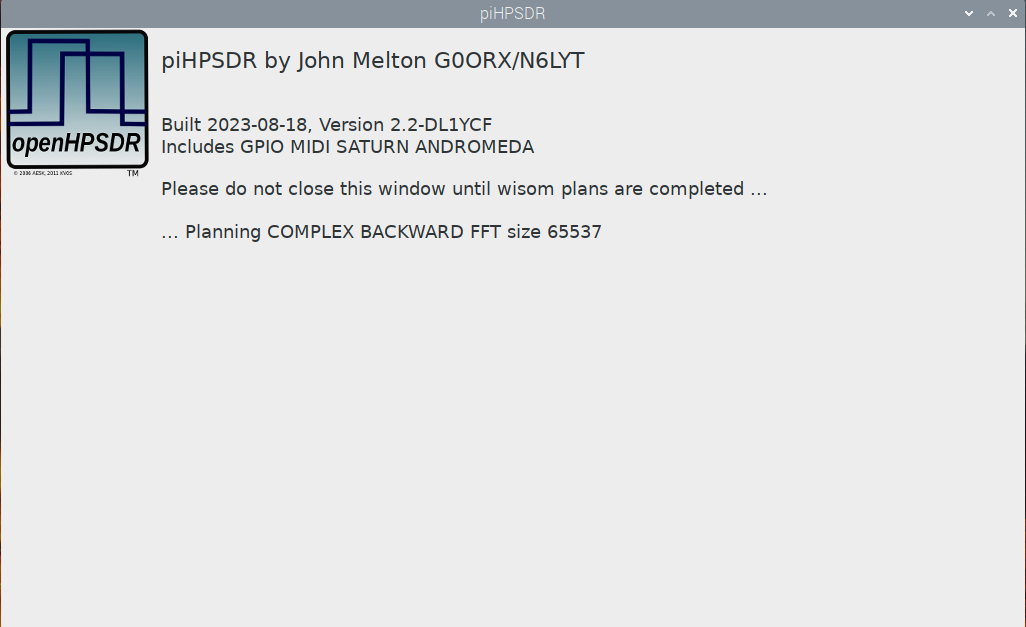
\includegraphics[width=12cm]{Planning.png}
\caption{piHPSDR screen while completing the ,,wisdom plans''.}
\label{fig:Planning}
\end{figure}

If the piHPSDR program is started for the first time, it opens a window that looks like Fig. \ref{fig:Planning}. 
Besides stating a version number and when piHPSDR was built, a list of optional features (to be activated
at compile time) is stated, in this case, GPIO, MIDI, SATURN, and ANDROMEDA. These options indicate
that the program has GPIO support (this is only possible on Raspberry Pi or similar single board computers),
that is has support for MIDI devices, that it can run natively on the compute module of the latest
G2 (generation two) SDRs from Apache labs, and that is has support for Laurence Barker's ANDROMEDA controller.
What is important here that you have to wait. This only applies to the very first time you start piHPSDR.
On CPUs with a rather simple instruction set (like the ARM processor in the Raspberry Pi, or the Apple
Silicon processor in recent Macintosh computers), this "planning" step is quite fast. For example, on my
Apple M2 Mac mini, this step takes six seconds. On the contrary, on CPUs with very
complex instruction sets like the Intel x86 processors, this step can last up to 15 minutes. But note
this has only to be done once, in subsequent starts of piHPSDR, the ,,wisdom'' will simply be read from
the file created during the ,,wisdom plans''.
When the ,,wisdom'' is secured, piHPSDR tries to detect a radio on the network. If everything went well with
the network connection, you then see a screen with a discovery menu (Fig. \ref{fig:Start}).

\begin{figure}
\center
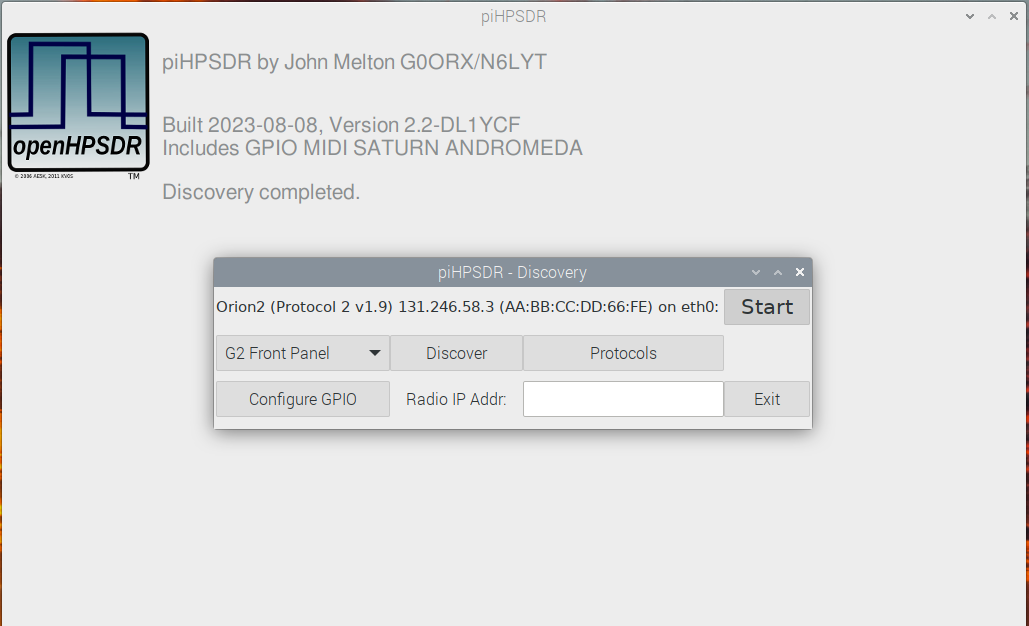
\includegraphics[width=12cm]{Start.png}
\caption{A radio has been discoverd. You are ready  to start it.}
\label{fig:Start}
\end{figure}

At this point, you can start the radio by clicking the \rett{Start} button, but let us first explain the
purpose of the other buttons! Easiest to explain is the \rett{Exit} button, this will simply terminate
the program. Most likely, you may want to go into the \rett{Protocols} menu sooner or later.
 By default, piHPSDR tries to
discover the presence of a radio using all protocols known to piHPSDR. However, if you know that your radio, for
example, uses P2 (Protocol 2), then trying to discover a P1 (Protocol 1) radio is just a waste of time. So if you
know which types of radio you want to connect to, you can enable (only) these in the \rett{Protocols} menu.
The available protocols are
\begin{itemize}[font=\texttt, left=80pt]
\item[Protocol 1]{This is the "original" HPSDR protocol.}
\item[Protocol 2]{This is the "new" HPSDR protocol.}
\item[Saturn XDMA]{This is used to talk to a Saturn FPGA through the internal XDMA interface. Only available
if piHPSDR is compiled with the \texttt{SATURN}  option.}
\item[USB OZY]{This is used to talk to a radio using the legacy USB OZY interface. Only available if piHPSDR
is compiled with the \texttt{USBOZY} option.}
\item[SoapySDR]{This is used to talk to a radio through the SoapySDR library, for example to an AdalmPLUTO. 
Only available if piHPSDR is compiled with the \texttt{SOAPYSDR} option.}
\item[STEMlab]{This is used to connect to RedPitaya based SDRs through the WEB interface. Only available if piHPSDR is
compiled with the \texttt{STEMLAB\_DISCOVERY} option. Starting the radio using this protocol is a two-step process:
first, the RedPitaya's WEB interface is located, and the \texttt{Start} button then starts the SDR app
on the RedPitaya. Then, piHPSDR tries to connect to this SDR app and upon success offers a new \texttt{Start} button
to start the radio. If the RedPitaya is exclusively used as a radio, it is recommended to auto-start the SDR app
when the RedPitaya is powered up. In this case, the STEMlab protocol is not used, because the SDR app can be started
through Protocol-2.}
\item[Autostart]{This is a very useful option. It indicates that if exactly one radio has been found, it is automatically
started. So in normal operation, when starting piHPSDR subsequently, and all settings are still valid, the radio is
started without user intervention. If this option is activated and one radio is present, you will not see this menu, so in order
to make further changes here, you have to disconnect the radio from the ethernet cable, start piHPSDR until you see this
menu, and reconnect the radio.}
\end{itemize}

Sometimes piHPSDR needs to know the IP address of the radio. This is, for example, the case for the \texttt{STEMlab} discovery
described above. In such a case the IP address in numerical form (xxx.xxx.xxx.xxx) can be entered in the box
with the label \rett{Radio IP Addr:}. If a legal IP address is contained in this box, protocol-1 and protocol-2 discoveries
will also send, in addition to a broadcast discovery packet, such a packet to the IP address specified. This way one can
connect to radios which are not on the same subnet as the computer, in principle you can connect to any radio on the world
provided it is on the internet. However, the original HPSDR standard states that a broadcast packet must be used, so several
radios won't reply. On the other hand, there are some radios such as a RedPitaya or a HermesLite-II which allow being discovered
by such a routed packet. 

The \rett{Discover} button re-starts the discovery process. This is useful if the radio has been powered up too late and
was not yet ready when piHPSDR was started. Simply press \rett{Discover} to give another try.

The combo-box (pop-down menu) to the left of the \rett{Discover} button lets you choose which type of GPIO controller you
have attached to the computer. This menu is only available if piHPSDR has been compiled with the \texttt{GPIO} option, which
is not the case on desktop/laptop computers. The menu lets you choose between

\begin{itemize}[font=\texttt, left=80pt]
\item[No Controller]{Choose this if no GPIO controller is wired to your Raspberry Pi.}
\item[Contoller1]{Choose this if you have a "version 1" piHPSDR controller.}
\item[Controller2 V1]{This option is valid for some early prototypes of the "version 2" controller with single encoders.}
\item[Controller2 V2]{Choose this if you have a "version 2" piHPSDR controller with double encocders.}
\item[G2 Front Panel]{Choose this if you have an ANAN G2 radio with a built-in controller.}
\end{itemize}

\textbf{Attention.} Be sure to choose a controller only if such a controller is actually connected to your Raspberry Pi. If
you choose, for example, a controller which uses an I2C expander for the switches, but no I2C interface is present on
your Raspberry Pi, the program my hang when trying to open the I2C connection.

All settings (protocols, controller, IP address) made in this menu are stored in the global (radio-indepentend) settings
and are restored when piHPSDR is started the next time. 

If all went well, a radio could be discovered and you hit the \rett{Start} button, the radio is started, and
if this succeeds, you see something like shown in Fig. \ref{fig:FirstDisplay}.

\begin{figure}
\center
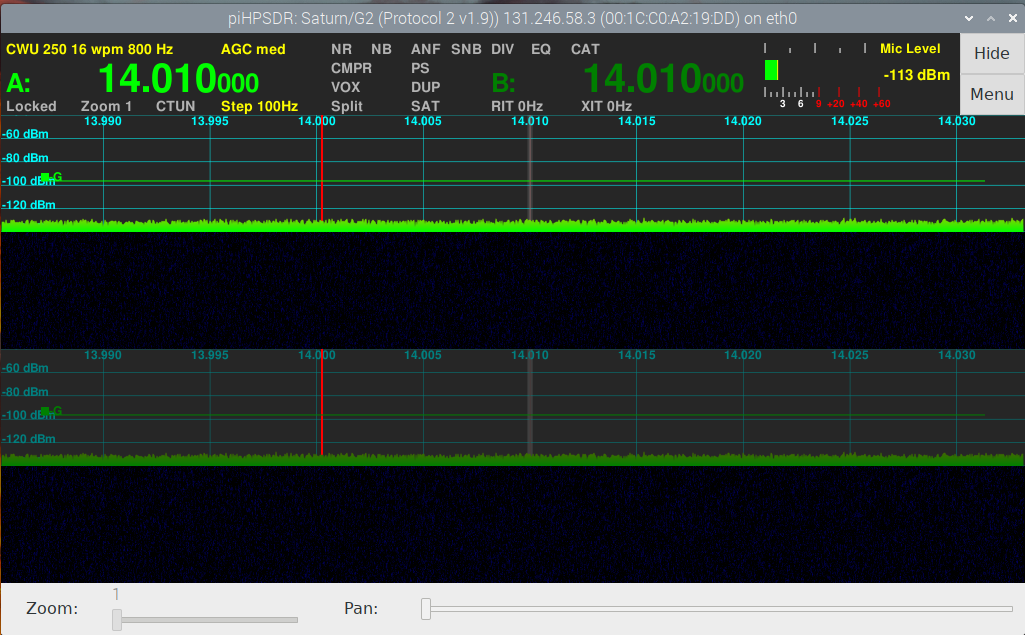
\includegraphics[width=12cm]{FirstDisplay.png}
\caption{The radio with two RX. Sliders and Toolbar are not on display
by default when using a controller.}
\label{fig:FirstDisplay}
\end{figure}

The bottom of the window looks different (more controls) if you have chosen \rett{No Controller} in the preceeding menu.
You see two receiver panels stacked vertically, both of them having a spectrum display and a waterfall area. At the top,
just below the window title, you have the VFO bar which contains information on the frequencies of the two VFOs A and B,
as well as lots of further information, to be explained later. At the top right, there are two buttons \rett{Hide}
and \rett{Menu} which will be explained in the next chapter. To the left of these two buttons, there is the meter
bar which by default is a digital S-meter. At this point, you have started piHPSDR successfully for the first time.

\chapter{Main window layout}

\section{One or two receivers}
At the end of the previous chapter (Fig. \ref{fig:FirstDisplay}),
 there were two receiver panels in the
piHPSDR window, stacked vertically, and both including a spectrum scope
(the green-coloured noise floor) and a waterfall. The waterfall area
is completely black in the above picture since there was no RF signal.
piHPSDR can be switched between having one or two receivers in the
\texttt{Radio} menu. If there are two receivers (called RX1 and RX2),
 one of the two is the \textit{active receiver}. If you look closely
 at the above picture, you will note that the spectrum scope of
 the lower (RX2) panel is shaded, while it is in bright colour for RX1.
 This indicates that RX1 is currently the active receiver. By simply
 clicking into the panel of the other (inactive) receiver, either with
 a mouse or on a touch screen, the formely inactive receiver becomes
 active.
 
 Many conventional rigs with two independent receivers discriminate
 between the "main" and the "sub" receiver. It is important that
 this is \textit{not} the case for piHPSDR. Both  receivers are
 largely equivalent. For example, if you start transmitting in
 normal (non-split) mode, the TX frequency matches the frequency
 of the active receiver, no matter whether this is RX1 or RX2.
 Likewise, in split mode, the TX frequency matches the frequency
 of the non-active receiver. Most of the receiver-specific controls,
 for example adjusting the AF volume or the AGC gain, refer to the
 current active receiver. If piHPSDR runs with two receivers,
 RX1 is always controlled by VFO-A while RX2 is controlled by VFO-B.
 The VFO settings not only include the frequency but also the
 current mode (e.g. LSB or CWU), the filter setting, the band and
 bandstack setting, whether RIT is enabled or not, and the RIT
 offset. So changing the RIT value only changes it for the active
 receiver. If you want  to change the RIT value for RX2 while RX1 is
 the active receiver, you have to make RX2 active, change the RIT
 value and then make RX1 active again.
 
 RX1 and RX2 are largely independent. They can receive on different
 bands. They can receive from different antennas provided the radio
 has two RF frontend with two analog-to-digital converter4s (ADC,
 as most modern radios do. In this case, one usually
 assigns the first ADC (ADC0) to RX1 and the second ADC (ADC1) to
 RX2. This can be done in the \texttt{RX} menu.
 
 By default, if there are two receivers, they are vertically stacked,
 with RX1 in the upper part and RX2 in the lower part of the display.
 This can be changed in the \texttt{Screen} menu to horizontal stacking,
 where RX1 is  in the left half and RX2 in the right half of  the 
 display. Changing the stacking trades vertical against horizontal
 resolution, of course.
 
  
\begin{figure}[h]
\center
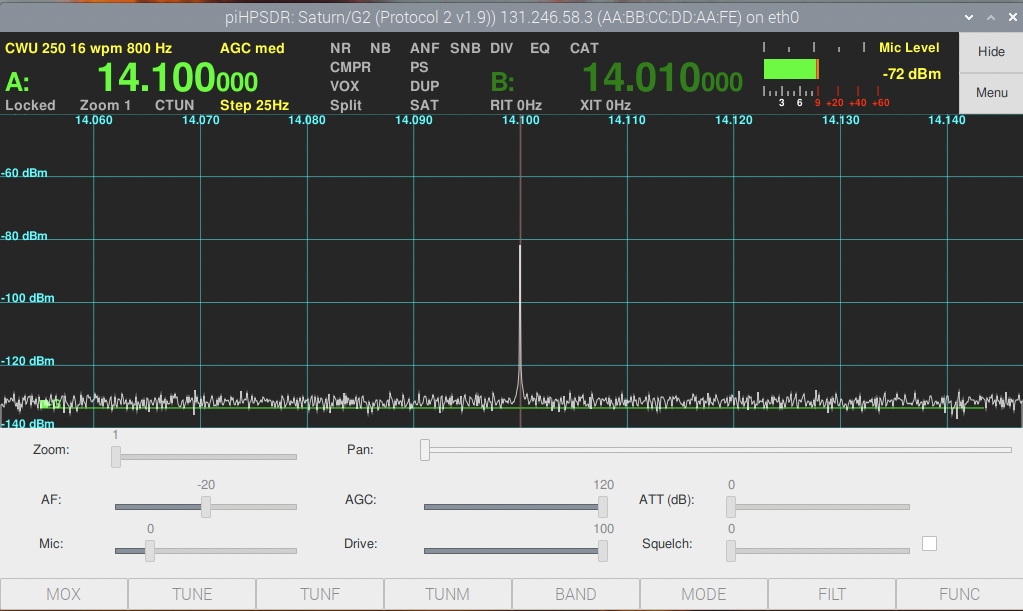
\includegraphics[width=12cm]{SingleReceiver.png}
\caption{piHPSDR with a single RX and all controls (Zoom/Pan,
Sliders, Toolbar) at the  bottom.}
\label{fig:SingleReceiver}
\end{figure}

 Fig. \ref{fig:SingleReceiver} picture shows, for demonstration purpose, a piHPSDR
 window with a single receiver. 
 The RX panel only contains a
 spectrum scope with a white line and no waterfall (this can be changed in the
 \texttt{Display} menu. In addition, you see the toolbar
 with eight buttons at the lower edge of the window, and above
 it an area with sliders. Showing the sliders is the default
 (and necessary) if there is no GPIO or MIDI controller attached,
 since then these sliders are the only way to change, for example,
 the AF volume. If there is only one receiver, it is controlled
 by VFO-A. VFO-B then actually controls nothing (except the TX
 frequency in split mode), but the data stored in VFO-B can
 be quickly used, for example by copying VFO-B to VFO-A (the
 \texttt{A<B} command), or by swapping the two VFOs (the
 \texttt{A<>B} command).

\section{Spectrum scope options}

You have already seen two different spectrum scopes: in the first
picture, the  spectrum was a filled green area, while in the last
picture, there only was a white line (this is similar to what you
would see on a spectrum analyzer). This can be adjusted to your
personal preference in the \texttt{Display} menu (see below). There
are two options which you can enable or disable, such that there
are four different outcomes. The first option is the ,,Filled'' option
which discriminates between a line spectrum and a spectrum which is
filled below the line. In the picture below, the first and third
example have no filling, while the second and fourth spectrum
are filled:

\begin{figure}[h]
\center
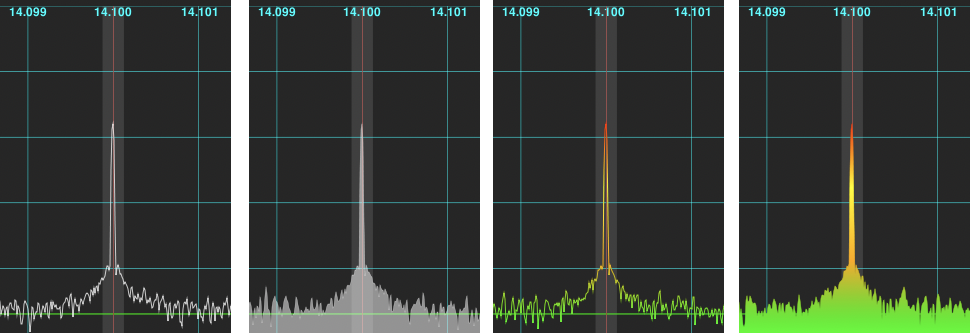
\includegraphics[width=12cm]{ScopeFilling.png}
\caption{Display options for the spectrum scope.}
\end{figure}

Then there is the ,,Gradient'' option. Without this option, the
spectrum is displayed in white colour. With the gradient option,
the colour changes from green over yellow towards red depending
on the signal strength (red colour is reached for S9). The above
picture demonstrates the four possible combinations, and in
the \texttt{Display} menu, you can make your choice. This setting
refers to both receivers when there are two. Note that the TX
spectrum can be a filled one or a line spectrum, but that the
gradient option does not apply.

\section{Zoom and Pan}

\begin{figure}[h]
\center
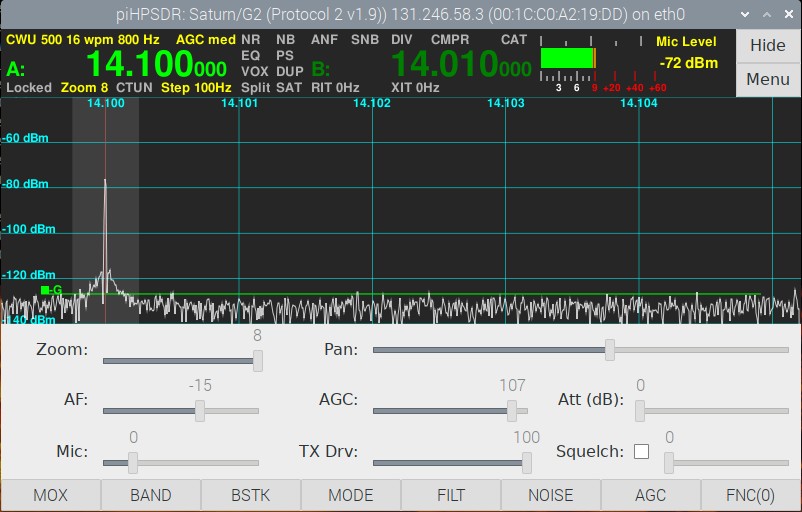
\includegraphics[width=12cm]{ZoomPan.png}
\caption{The spectrum scope of Fig. \ref{fig:SingleReceiver} with a
large Zoom value.}
\end{figure}

The width of the RX spectrum equals the sample rate
of the receiver. This means that if you use, say,
a sample rate of 96 kHz for a receiver, its spectrum
will be 96 kHz wide, which may encompass a larger part
of the spectrum than you are interested in. As a drawback,
the part which is relevant to you may look a little bit
compressed. This is where the \rett{Zoom} function
comes in. The zoom value can adopt integral values between
1 (no zoom) and 8. In the latter case, only 1/8 of the
overall spectrum is displayed on the screen. In the
picture below, you see that the RX scope is only 12 kHz
wide (which is 1/8 of the RX sample rate, 96 kHz in our
example). Note that what is displayed is in full resolution.
Internally, a spectrum with 8 times the number of pixels
of the screen width is created and only a part of it is
displayed. The zoom value can be changed using the \rett{Zoom}
slider (at the left edge below the RX panel).


When using a zoom value larger than one, this means that
a spectrum with more pixels than the actual screen width
is produced. One can select which part of that area
is displayed on the screen with the \rett{Pan} slider
(below the RX panel at the right side). Normally (Zoom=1),
the VFO dial frequency is exactly in the middle of the
RX scope, and marked with a thin red line. On the picture
above, the dial frequency (14.100 MHz) is found in the RX
panel close to the left edge, and this has been done
by moving the \rett{Pan} slider.

\section{The \texttt{Hide} button}
\begin{figure}[h]
\center
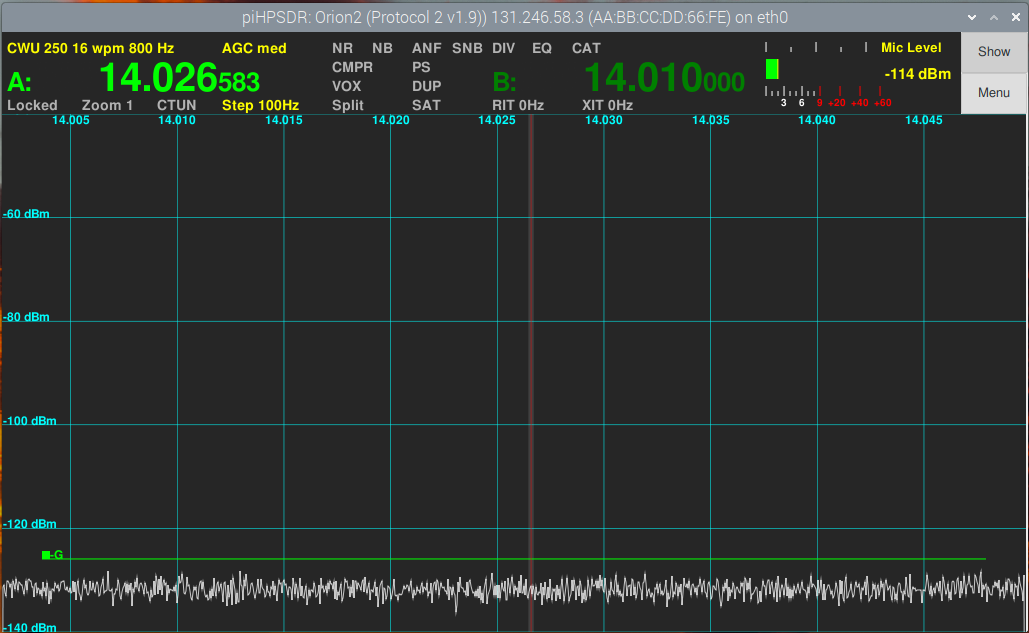
\includegraphics[width=12cm]{Hidden.png}
\caption{piHPSDR window with the Toolbar/Sliders/Zoom
area ,,hidden''.}
\end{figure}

On small screens, space is scarce. This in in particular true
for the vertical space if one used two RX panels and both
with a spectrum scope and a waterfall. I this case, it may be
hard to actually watch the signals if the screen is small.
This is where the \rett{Hide} button comes in. Clicking on
this button ,,hides'' the toolbar and slider area:


The text on the button then changes to \rett{Show}, and
clicking this button again will then return to the
previous display.

\section{Window areas}

Look again at Fig. \ref{fig:SingleReceiver}! Starting from the
top, you see the title bar of the window. This bar is not visible
in full screen mode, where the size of the piHPSDR window matches
the display size. The title bar contains some basis information
about the radio, e.g.  its type, the protocol used, the  IP
and the hardware address of the radio. If you are really interested
in this information, it is recommended to open the
\texttt{About} menu.

Between the title bar and the RX spectrum scope, you see
a small vertical area, most of  which is taken by the VFO bar
(containing the large frequency dials). At the rightmost
end of this area, you see two buttons \rett{Hide} (already
discussed) and \rett{Menu}. Clicking on the latter button opens
the main menu, which will be discussed in detail in the following
chapters. The \rett{Menu} button is really important, since it
enables access to one of the menus used for configuring piHPSDR.
Between the VFO bar and the \rett{Hide}/\rett{Menu} buttons,
you see the meter area where you find the S-meter (during RX)
and information about output power, SWR, etc. during TX.

Below the RX  spectrum scope, you see the Zoom/Pan area with
the  Zoom and Pan sliders, as already discussed. This area
can be ,,hidden'' with the \texttt{Display} menu to save some
vertical space. Below the
Zoom/Pan sliders you see a larger  Sliders area containing
several sliders for adjusting AF volume, TX  drive leve, 
RX  AGC threshold, etc. Although the Sliders area can also
be hidden via the \texttt{Display} menu, you should not do so
unless you have a GPIO or MIDI controller which knobs that
you can asssign to the slider functions. This is so since
for  normal operation, having access to the sliders is vital.
Remember that for temporarily enlarging the space for
the RX  panel, there is the \rett{Hide} button!

\begin{figure}
\center
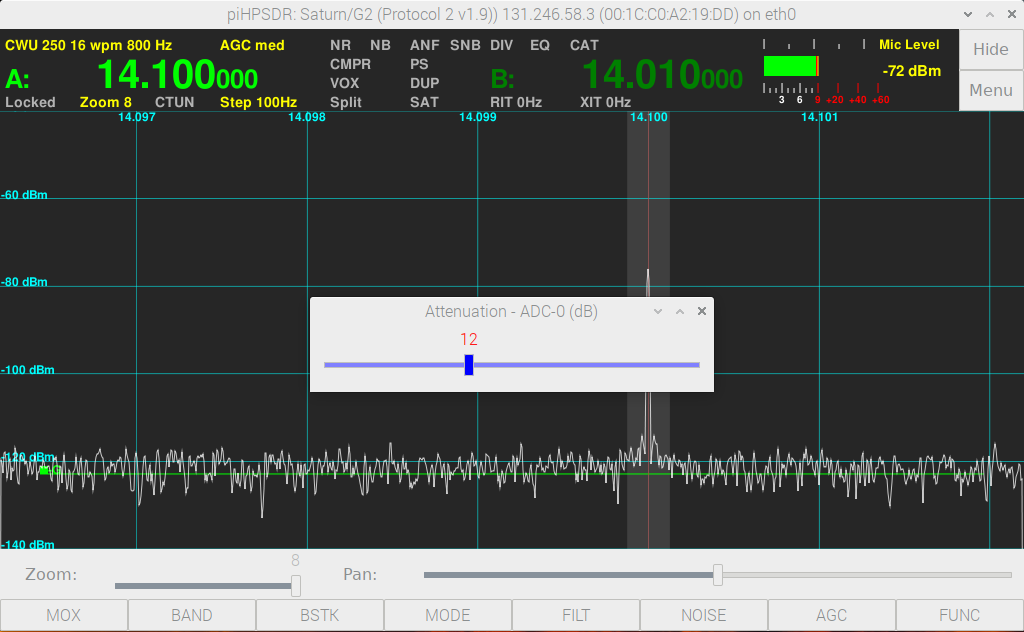
\includegraphics[width=12cm]{SliderOnScreen.png}
\caption{A pop-up attenuation slider.}
\label{fig:SliderOnScreen}
\end{figure}

If you have a GPIO or  MIDI  console, and, say, assigned
a knob there to control the AF volume, then turning the
knob will auto-magically also move the AF slider if its
on display (that is, if the sliders area is not hidden).
If you turn a knob for which function there is slider
on display, either because the slider area is hidden or
because this function does not have a slider in that area,
then a graphical slider will temporarily pop up in the
middle of the window to inform you about the changes 
you have  made. To give one example, a knob at a
MIDI console has been assigned to the RF attenuator (\texttt{ATTEN}
function, see Appendix A), which controls the step 
attenuator in the RF front-end (if there is one). As long
as the  sliders  are  on display, the \texttt{Att} slider
in the left part of the slider area moves when turning
the knob. But when the sliders are not displayed, then a slider image
pops up  on the middle of the screen, and the
bar contained therein moves when turning the knob,
and the numerical value is displayed as well (Fig. \ref{fig:SliderOnScreen}).
Such a pop-up slider always occurs if a knob on the GPIO or MIDI
console is turned and no slider associated with the value changing is
on display.


\section{Mouse clicks in the main window}
The main window ,,accepts'' mouse or touchscreen click events.
Some of them come from the standard handlers of the GUI. It is
clear, for example, that clicking the \rett{Hide} or
\rett{Menu} buttons, as well as clicking one of the
toolbar buttons, will activate the function associated with
these buttons. Furthermore, the sliders (and the squelch enable/disable
checkbox) in the sliders and Zoom/Pan are are operated as usual.
But there are additional functions coded into piHPSDR:

If there are two receivers, a mouse click (press and release) into
the panel of the non-active receiver makes it active. On the other
hand, a mouse click in the panel of the active receiver changes
the VFO frequency of that receiver to the value clicked on.
This means, if you see a signal in the spectrum scope, click
on that signal and your VFO will move (,,jump'') to that signal.
Note the VFO frequency will be  rounded to the next multiple of
the VFO step size when ,,jumping'' by a mouse  click or
touch screen press.

The second option to change the VFO frequency of the active receiver
is to click (and hold) into its panel, then drag the mouse to the left
or to the right, and then release the button. This will shift the
VFO frequency by the amount dragged, it makes no difference 
where the first click actually occured, only the difference
in horizontal position between click and release is used. You must
drag at least three pixels so there is clear discrimination between
a ,,VFO jump'' (click then release) and a ,,VFO drag'' (click, drag,
and release) operation. Finally, the VFO frequency of the active
receiver can be changed by the scroll wheel of the mouse, if there
is any. Using the scroll wheel lets the VFO frequency move in multiples
of the VFO step size, while mouse dragging can also be used for
finer tuning.

Clicking into the VFO bar opens the \texttt{FREQ} (VFO) menu,
for the VFO-A if clicked into the left half of the bar, and for
VFO-B if clicked into the right half. This menu not only offers
the possibility for direct frequency entry, but also lets you 
alter the RIT/XIT or VFO step size, or alter the Lock, Duplex,
CTUN, or Split states. So a simple click in the VFO bar 
gets you quick access to often-used functions.

Clicking in the meter section (between the VFO bar and the
Hide/Menu buttons) opens the \texttt{METER} menu, where
you can change the meter properties (see below).

When operating with a mouse, there are usually two mouse buttons,
the primary button (for right-handed mouses, this is usually
the left button) and a secondary one. Secondary mouse clicks
are difficult to apply with a touch-screen. Although there are
touch-screen drivers which convert long presses to secondary clicks,
they generate, for a long press, a primary click first and a
secondary one later, so it is not possible to generate a
single ,,secondary press'' event. But for the benefit of
mouse users, secondary mouse clicks are handled in a special way:

A secondary click into the VFO bar will open the \texttt{BAND} menu,
so a band change can be made with really few mouse clicks. Likewise,
a secondary click into the panel of a receiver (no matter if it
the active or the non-active one) will open the \texttt{RX} menu
for that receiver. This can be used to change the settings of a
non-active receiver without making it temporarily active. In the
same way, a secondary click in the TX panel will open the
\texttt{TX} menu.

\section{VFO bar and status  indicators}
\begin{figure}[h]
\center
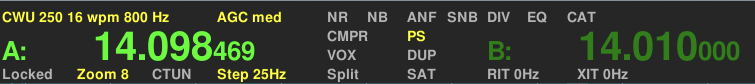
\includegraphics[width=12cm]{VFObar.png}
\caption{The VFO bar}
\label{fig:VFObar}
\end{figure}

Fig. \ref{fig:VFObar} shows the VFO bar layout in more  detail.
The example shown is a VFO bar whose width is 745 pixels and
thus suitable for screens that are 1024 pixels wide (or more),
since the meter area has a fixed width of 200 pixels, and
the \texttt{Hide/Menu} buttons are 65 pixels wide. This layout is
denoted \texttt{Large dials for 1024px windows}, as to the choice
of VFO bar layouts, see the description of the \texttt{Screen} menu.

The large dials indicating the frequencies of VFO-A and VFO-B
are easily recognized. The number to the left of the decimal
point is the MHz part of the frequency, the three  large digits
to the right  of  the decimal point is the kHz part, and
the last three (smaller) digits offer sub-kHz resolution.
You may wonder why there is  so much space to the left of
the frequencies. This is so because with the advent of
the QO-100 satellite, frequencies above 10 GHz can be
used (with the transverter bands) and therefore eleven
digits are needed!

Apart from the frequencies, you see a lot  of text, most in
light grey colour. As a general rule, a text  in grey
colour indicates a feature that is currently disabled,
while features currently active are normally shown in
yellow and sometimes in red.

At the top left  corner of the VFO bar, the mode and
filter of the currently active receiver is displayed. 
In Fig. \ref{fig:VFObar}, the text is \texttt{USB Var1}
which indicates that the  mode
is USB using the Var1 filter with variable width (see the \texttt{Filter} menu).
For the CW (CWU and CWL) modes, the CW speed (in wpm) and the side tone
frequency (in Hz) is stated as well.

Now we continue line by line, from left to right and find
the string \texttt{AGC med} printed in yellow. This means
that automatic gain control (AGC)  is effective  in the
active receiver, and that the AGC time constant is
intermediate. Possible values for the time constant 
are Long, Slow, Medium and Fast which can be selected
in the \texttt{AGC} menu. Here one can  also disable AGC,
in this case the VFO bar shows \texttt{AGC off} in grey
colour.

Continuing to the left, we see the noise reduction settings,
all printed in grey (that is, they are not effective). This
can be changed in the \texttt{Noise} menu. We have two different
noise reduction capabilities \texttt{NR1} and \texttt{NR2}, these
strings are printed in yellow instead of the grey \texttt{NR} if
they are effective. There are also two different noise blankers
\texttt{NB1} and \texttt{NB2}, the automatic notch  filter
\texttt{ANF} and the spectral  noise blanker \texttt{SNB}.
Besides enabling/disabling these functions, there are  further parameters
you can tweak in the \texttt{Noise} menu.

The next strings whether Diversity reception is enabled or disabled
(\texttt{DIV}), or whether an equalizer is effective \texttt{EQ}.
Since there is a separate equalizer for the RX and TX audio chain,
the equalizer indicator, if it is effective, not only turns yellow
but reads \texttt{RXEQ} while receiving and \texttt{TXEQ} while
transmitting. This means, if only the TX equalizer is enabled,
the indicator will show a  grey \texttt{EQ} while receiving
and a yellow \texttt{TXEQ}  while  transmitting.

The last indicator in the top row  is \texttt{CAT} which indicates
if the CAT module  (see the \texttt{RIGCTL}  menu) has accepted at least
one connection. In total, piHPSDR can be CAT-controlled simultaneously
by five different sources, two of them using a serial line and
three of them a TCP connection. 

The indicators in the middle, between the VFO dials, are related to
transmitting. \texttt{CMPR} indicates if a speech processor
(compressor) is enabled, if so, it prints in yellow, followed
by a number between 1 and 20 indicating the compression value in dB.
\texttt{PS} indicates whether adaptive pre-distortion (,,PureSignal'')
is enabled, PS settings can be made in the \texttt{PS} menu.
 \texttt{VOX} indicates whether VOX (voice control) is enabled. VOX means
 that if  the microphone delivers an amplitude above a certain threshold,
 the radio is automatically put into TX mode. Enabling/Disabling VOX
 and setting the correct threshold can be done in the \texttt{VOX} menu.
 Finally, \texttt{DUP} indicates whether duplex mode is active.
 In duplex mode, the receiver(s) continue to work during transmit. Duplex
 mode when using the same antenna for RX and TX is  no fun: you not only hear
 your own signal with a delay (from the cross-talk at the TRX relay), but
 this cross-talk signal is  usually so strong that it leads to ,,AGC pumping'', so
 your receiver is virtually deaf during the first second after TX/RX
 transition. For satellite operation, on the other hand, duplex  mode
 is very convenient. Here you usually have two separate and well-decoupled
 antennas for RX and TX.
 
 The bottom line of the VFO bar  indicators are related to the VFO status.
 If the \texttt{Locked} string is red, it indicates that the VFO is locked
 and will not accept changes. There is a LOCK action which toggles the
 LOCK status and which can be assigned to a toolbar button or a push-button
 on a GPIO or MIDI console, but the Lock status can also be set/unset
 via the \texttt{VFO menu}.
 
The next indicator in the bottom  line indicates the Zoom factor. If the
Zoom factor is 1, the indicator is grey, otherwise it is yellow and
also indicates the factor. Then there is a string \texttt{CTUN} which
indicates whether the CTUN (,,click to tune'') mode is off or on (the string 
is yellow in the latter case). The step size of the VFO controlling the
active receiver is displayed next, this string is always yellow.

The split status is displayed by the next indicator, which is red in
split mode. If split mode is off, transmitting is done on the frequency
and the mode of the active receiver (if there are two receivers), or
on the frequency/mode of VFO-A (if there is only one receiver). If
split mode is on, transmitting occurs on the frequency/mode of the
non-active receiver (if there are 2) or on VFO-B (if there is only  one
receiver).

The next indicator shows the SAT (satellite) mode, which can be off
(then the indicator reads SAT in grey), or which can be SAT or RSAT
(then the indicator displays this  string). Once SAT mode is engaged,
the two VFOs are tied together such that any frequency change of one
of the two VFOs also applies to the other VFO. This is the best way
to do cross-band operation with, e.g. the QO-100 satellite which is at
a fixed position. In RSAT mode, a frequency change of one of the VFOs
is applied to the other VFO with an opposite sign (so if you move up
VFO-A by 2 kHZ, then VFO-B moves down by the same amount). This is
what one needs for low-flying satellites which have inverting
transponders which offer some sort of Doppler correction.

Finally there are the RIT (receiver incremental tuning) and XIT
(transmitter incremental tuning) indicators. If RIT is off,
receiving occurs on the VFO dial frequency. If RIT is on, the 
indicator becomes yellow and also indicates the RIT offset, that is,
the frequency offset used while receiving. RIT is used, for example,
if during your CW QSO the frequency of the transmitter of your
QSO partner drifts and you want to follow without altering the
frequency of your own transmitted signal. The RIT indicator
corresponds to the active receiver. If XIT is active, the
indicator becomes yellow and shows the offset of the ,,true''
TX frequency from the VFO dial frequency. 

Finally, in the top right corner you see a symbol with a green and a red line
that only occurs if
one of the variable filters (\texttt{Var1} or \texttt{Var2}) have been
selected. The green caret indicates the default filter edges,  while the
red one above denotes the current filter edges. 

\section{Meter section}

Fig. \ref{fig:MeterDesigns} shows the different designs that exist for
the meter. To the left (right) there are the digital (analog) meters,
while the top panels show the meter during RX and the lower panels
during TX.

\begin{figure}[h]
\center
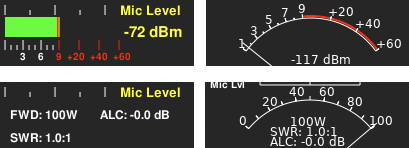
\includegraphics[width=8cm]{MeterDesigns.png}
\caption{Different designs for the meter.}
\label{fig:MeterDesigns}
\end{figure}

The design can be switched between digital and analog in the \texttt{Meter}
menu, which can be accessed quickly just by clicking into the meter area.
During RX, an S-meter is shown together with the signal level in dBm. Note
that -73 dBm corresponds to S9 for frequencies up to 30 MHz, while above
30 MHz, S9 corresponds to -93 dBm. Since the S meter is in steps of
6 dB, a signal level of S1 (below 30 MHz) corresponds to -121 dBm.

During TX, the output power is displayed, provided that the radio actually
reports this power. The output power meter can be calibrated (see the \texttt{PA}
menu). If the SWR exceeds a threshold for SWR warnings (the default is 1:3, but
this can be changed in the \texttt{TX} menu), the SWR indicator turns red. If, 
in addition, SWR protection is enabled in the \texttt{TX} menu, the output
drived  will be reduced to zero if the SWR exceed that threshold.
Furthermore, the ALC (automatic level control) value of the transmitter is 
shown. Negative ALC values (at least in peak mode) indicate that the volume of the TX input audio
could be increased to get full output  power.

Further info on the meters (e.g. switching between ,,peak'' and ,,average'' reporting)
is described in the \texttt{Meter} menu.

\chapter{The Main Menu: introduction}

\begin{figure}[h]
\center
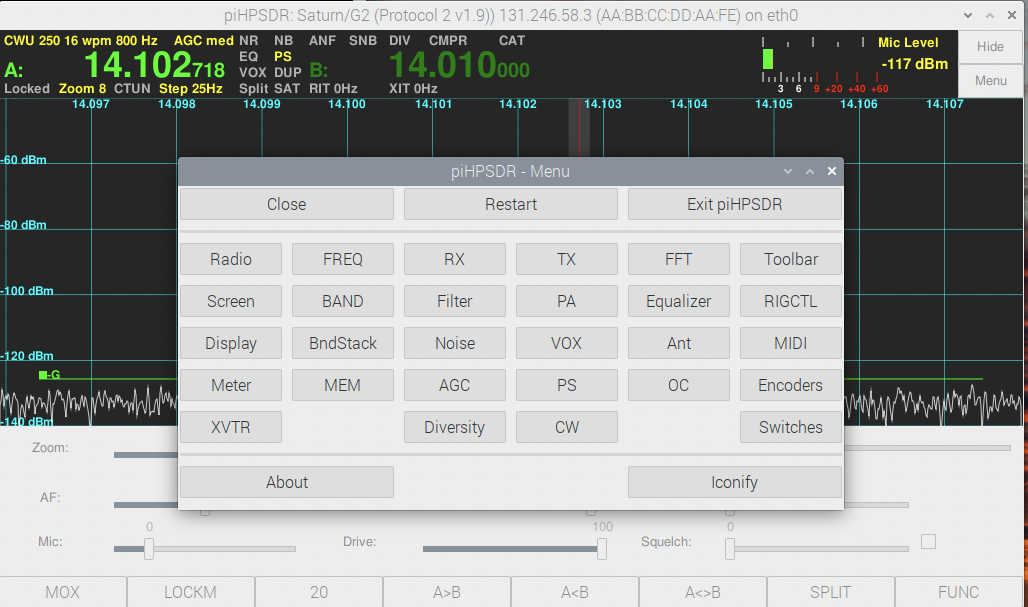
\includegraphics[width=12cm]{MainMenu.png}
\caption{The Main men, opened by the \texttt{Menu} button.}
\label{fig:MainMenu}
\end{figure}

Now we have a series of chapters that discuss all the piHPDSR menus. Many menus can be
opened by a "button" action, e.g. hitting the "MODE", "FILT", or "NOISE" button on the
toolbar you have seen in the last picture. You already know that the VFO and Meter
menus can be opened by clicking into the VFO or meter section at the top of the window.
When operating with a mouse, a secondary click in the RX or TX panadapter opens the
RX or TX menu. But there is one place from which \textit{all} piHPSDR menus are at hand,
and this is the "Main Menu". It can be opened by clicking into the "Menu" button at the
top right corne of the piHPSDR window, the outcome is shown in Fig. \ref{fig:MainMenu}.

Some remarks have to be made about menus in general. Since piHPSDR is optimized for
working with small screens, only one menu can be open at a time. If a menu is open
and one tries to open another one, the first menu will be destroyed (closed) and the
new one will be opened. For example, if you hit the \texttt{FILT} button in the toolbar
when starting from Fig. \ref{fig:MainMenu}, the main menu closes and the Filter menu
opens. If you try to open a menu that is already open, then the menu will be closed.
So, starting from Fig. \ref{fig:MainMenu} hitting the "Menu" button again will close
the menu. Likewise, when the Filter menu has been opened, either via the Main Menu
or with the \texttt{FILT} button, then hitting this button again will close the menu.

While the menus are looking quite diverse, some effort has been invested to keep
some things consistent throughout. For example, at the top left corner of the menu
you usually find the "Close" button which closes the menu. The close button is somewht
emphasised (slightly larger letters, and a thin border) so you will always quickly find it.
Of course, it it possible to close a menu by deleting the menu window (on RaspberryPi,
this is the small cross at the left of the title bar) but this is neither necessary nor
recommended.

There are some commands available here that do not directly affect the radio operation,
so these commands are found in the top and bottom line of the Main Menu. We first 
mention the \texttt{Restart} button in the middle of the top line. This restarts the
radio protocol. While not needed under normal circumstances, it my happen (especially
with beta releases of radio FPGA firmware) that the data exchange between piHPSDR and
the radio gets out-of-sync. I observed such problems with early versions of the P2
firmware for Orion2 boards and that is the reason the \texttt{Restart} button is
there, since this made a quick recovery possible without loosing the QSO.
At the bottom right, there is the \texttt{Iconify} button which ,,minimizes'' the
piHPSDR window. Normally, if needed, one can do so by standard methods of the
operating system in the title bar of the piHPSDR window. If piHPSDR, however,
runs in full-screen mode (this is the case on very small touch screens), then the
\texttt{Iconify} button to make the piHPSDR window temporarily disappear without
breaking the connetion to the radio, do some work with the operating system, and
get the piHPSDR window back. Note in earlier versions of piHPSDR this function was
associated with the "Hide" button in the top right corner of the main window.
Then, there are two menus ("Exit" and "About") which are described in due course and which
one can open by clicking either "Exit piHPDSR" or "About" in the main menu.

The other buttons, between the two horizontal separator lines, give access to piHPSDR
control and fine tuning. They are organized in six columns, namely radio related
menus (first column), VFO related menus (second column), RX and TX related menus (third
and fourth column), menus affecting both RX and TX (fifth column) and, finally,
menus for adjusting how you can control piHPSDR (sixth column), either via Toolbar,
MIDI, or GPIO encoders or switches. \textbf{,,Encoders''} are knobs which you can turn, and which
can be used to change AF volume or TX output power. \textbf{,,Switches''} are push-buttons which
can be used to trigger a function such as transmitting a carrier for tuning, toggle
between RX and TX, open a menu, and so forth.


\section{The \texttt{Exit} Menu}

\begin{figure}[h]
\center
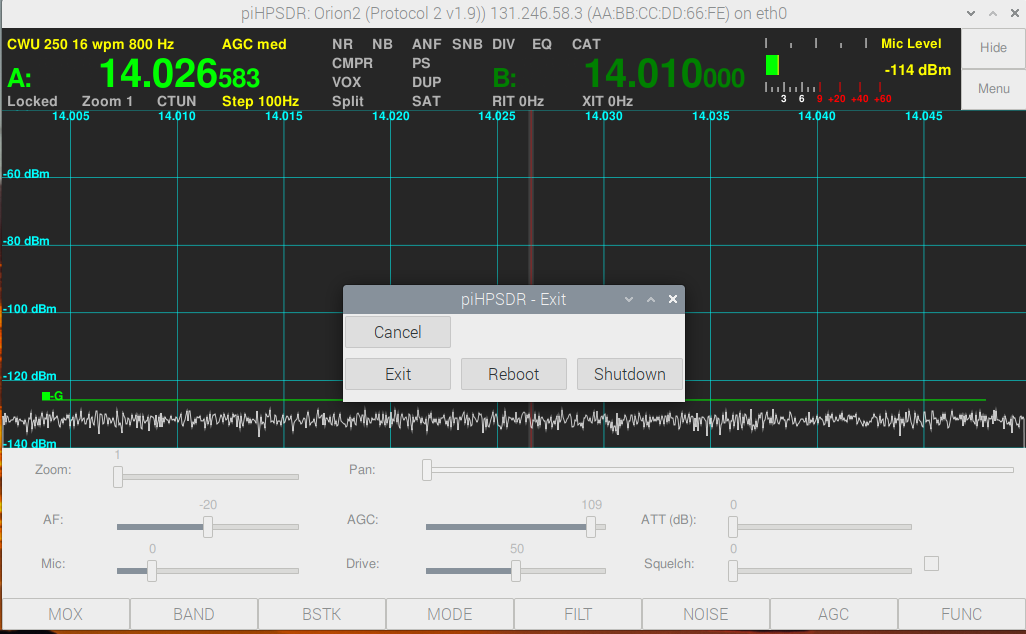
\includegraphics[width=12cm]{ExitMenu.png}
\caption{The \texttt{Exit} menu.}
\end{figure}

Via the \texttt{Exit} menu, you can leave the piHPSDR program. When leaving the program,
the radio protocol is stopped and all the settings are written to a preferences file. This
file is located in the piHPSDR directory and takes the name xx-xx-xx-xx-xx-xx.progs, where
the xx encode the MAC address for the radio. So the preferences for different radios (if you
have more than one) are stored in different files. To leave the program, just click the
"Exit" button in this menu. If you decide you want to continue, you can leave the \texttt{Exit}
menu by clicking the "Cancel" button. This is the button which closes the menu and has
the same position and look as the "Close" buttons in all the other menus.

If piHPSDR runs with administrator privileges, you can even leave the program and either re-boot
or switch off the computer via the "Reboot" and "Shutdown" buttons. This makes sense for setups 
where a Raspberry Pi running piHPSDR, a small SDR radio, a touch-screen and several encoders
and switches are built into a single common enclosure. On the other hand, when running
piHPSDR on desktop or laptop computers, clicking "Reboot" or "Shutdown" both leave the piHPSDR
program but no re-boot or shutdown takes place, due to missing administrator privileges.

\section{The \texttt{About} Menu}


\begin{figure}[h]
\center
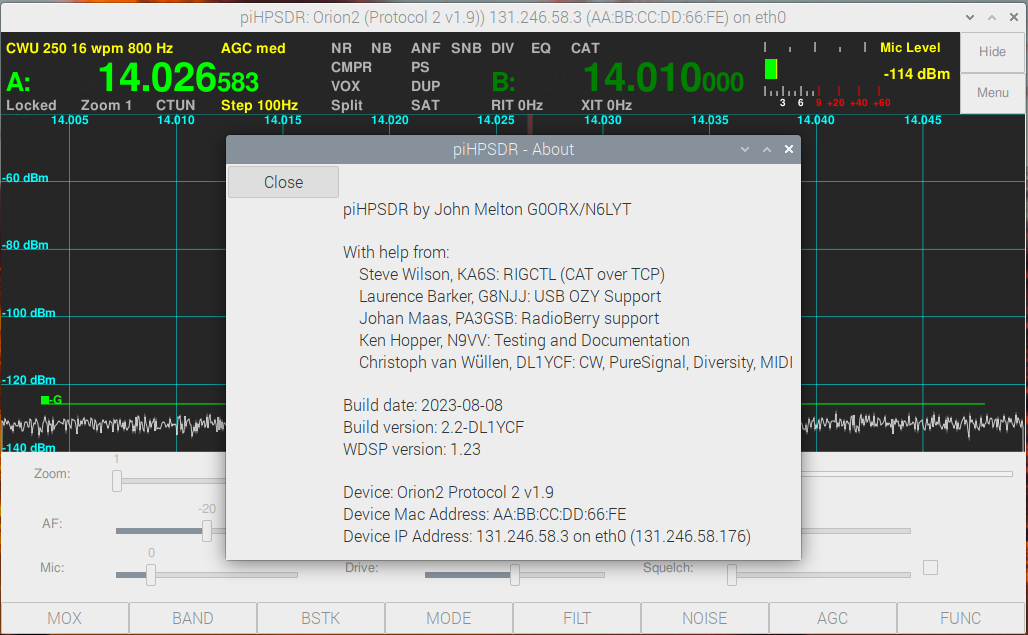
\includegraphics[width=12cm]{AboutMenu.png}
\caption{The \texttt{About} menu.}
\end{figure}

The about menu gives you some information about piHPSDR, first the original author
and an (incomplete) list
of persons who contributed to the code, and then a statement which version of piHPSDR
is working here, and when it has been compiled. Here you also find the version number of the WDSP
 library which is the ,,engine''
running under the hood, and which does nearly all of the signal processing. Finally, there is
some data on the radio, namely the device type and version numbers, and which protocol is running.
For diagnostic purposes, you also see the MAC address of the radio, its IP address and the
IP address of the computer running piHPSDR. The MAC address is of interest since the radio-specific
preferences are stored in a file whose name is derived from the radio's MAC address.

\chapter{The Main Menu: Radio-related menus}
\section{The \texttt{Radio} Menu}
\begin{figure}[h]
\center
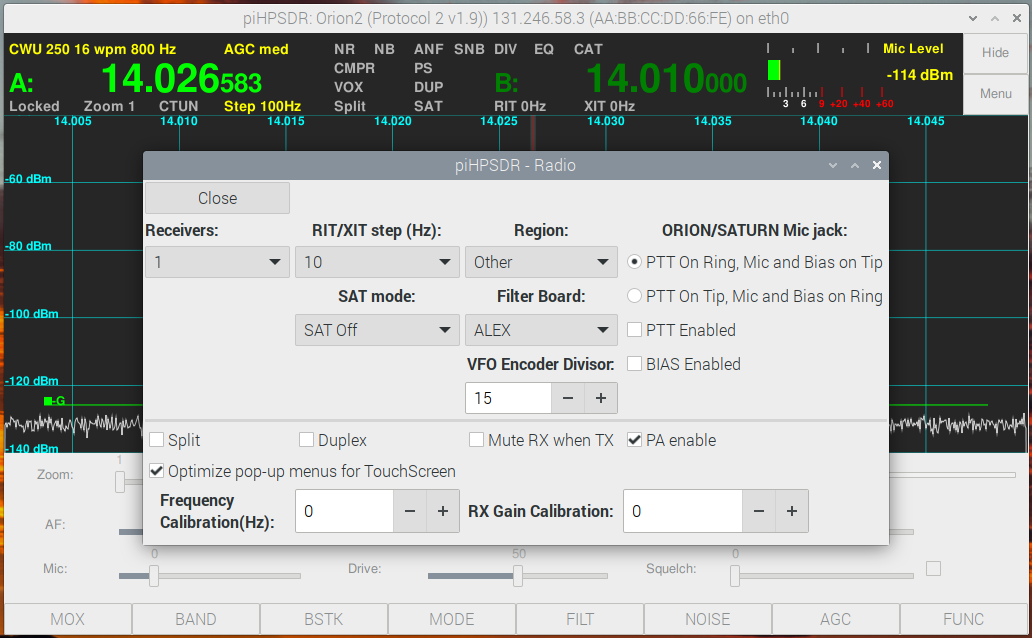
\includegraphics[width=12cm]{RadioMenu.png}
\caption{The \texttt{Radio} menu.}
\label{fig:RadioMenu}
\end{figure}


The Radio menu lets you make settings which affect the general setting, and the hardware of the radio.
The following figure (Fig. \ref{fig:RadioMenu}) shows the menu as it opens on an Anan G2 radio.
Note this menu looks slightly different for different radios and protocols, this will be discussed
at the end of the section. First, we go through all the elements we see in Fig. \ref{fig:RadioMenu},
they will be colored red in the following list.

\rett{Receivers.} In the pop-down menu (GTK combo-box) below this string, you can select the number
of receivers that are running (well, you can choose between 1 and 2). When the number of receivers change,
the radio communication will shortly be stopped and then resumed, so do not be surprised if the spectrum
scope freezes for a second or so.

\rett{RIT/XIT step.} In the pop-down menu you can choose among three (1 Hz, 10 Hz, 100 Hz) step sizes
for RIT and XIT. For example, if the RIT step is 10 Hz, then you can change the RIT offset in steps of
10 Hz with the RIT+ or RIT- buttons in the toolbar or on the GPIO/MIDI controller.

\rett{Region.} Although not obvious, this selects settings for the 60m band. Possible choices are "Other",
"US", "UK" and "WRC15". The US and UK choices implement the channel structure of the 60m band according
to the regulations valid in these countries. "WRC15" gives you a small (15 kHz wide) 60m band according to the WRC15
(World Radio Conference 2015) document, which is now implemented in many countries. With "Other" you
have a large 60m band from 5250 o 5450 kHz, but it is most likely not legal for you to operate in this
entire range.

\rett{Orion/Saturn Mic jack.} Modern radios can switch the connections of the TRS microphone jack in software.
While the ring of the TRS plug is always connected to ground, the microphone and PTT connections are on the
ring an tip and you can choose which one is on the ring and which one on the tip. You can then separately
enable the PTT function of the jack, and select whether a bias (DC offset) is applied to the mic connetion
(this is necessary for condensor microphones and detrimental if a dynamic mirophone is connected without
a blocking capacitor).

\section{The \texttt{Screen} Menu}

\begin{figure}[h]
\center
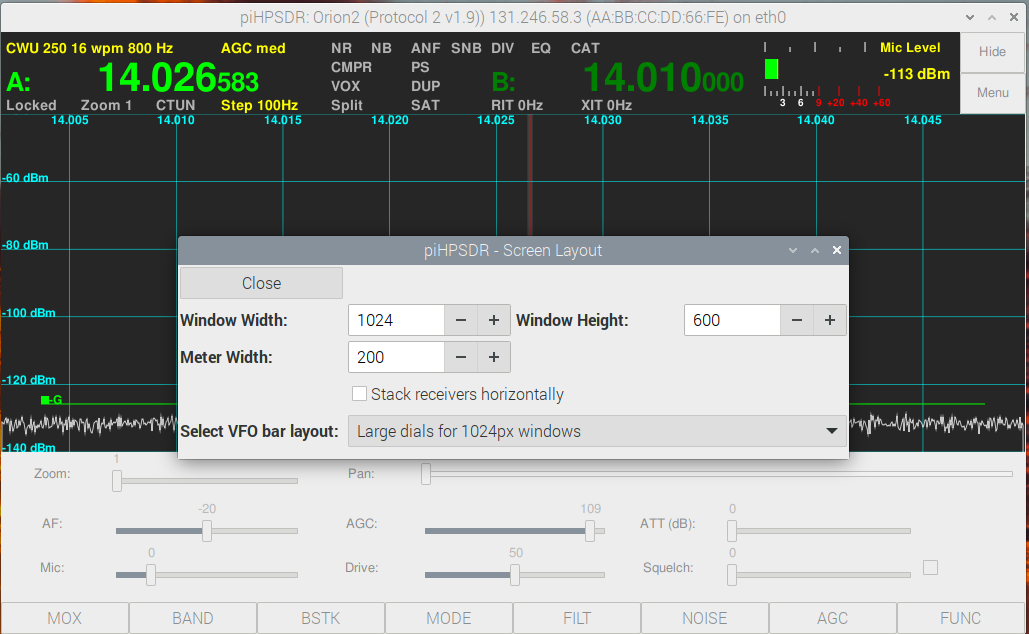
\includegraphics[width=12cm]{ScreenMenu.png}
\caption{The \texttt{Screen} menu.}
\end{figure}

\begin{figure}[h]
\center
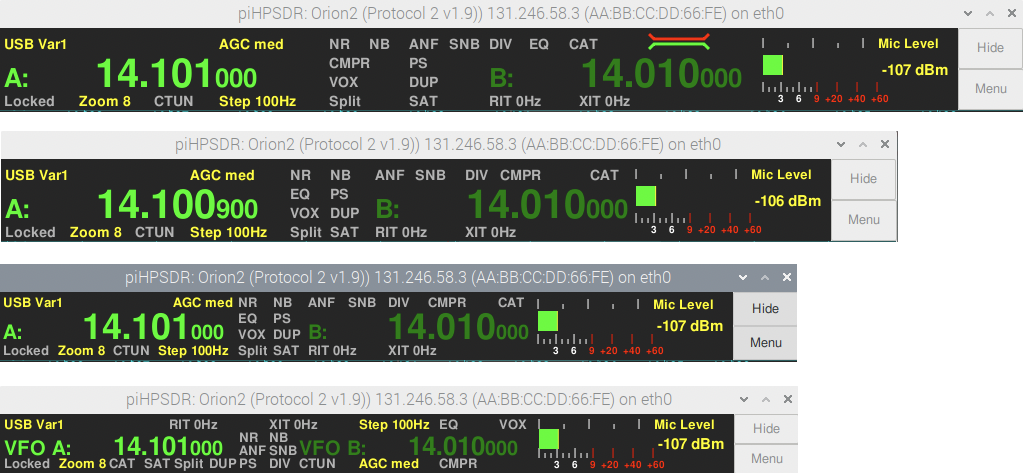
\includegraphics[width=12cm]{VFObarChoice.png}
\caption{Four choices for the VFO bar built into piHPSDR.}
\label{fig:VFObarChoice}
\end{figure}

\section{The \texttt{Display} Menu}
\begin{center}
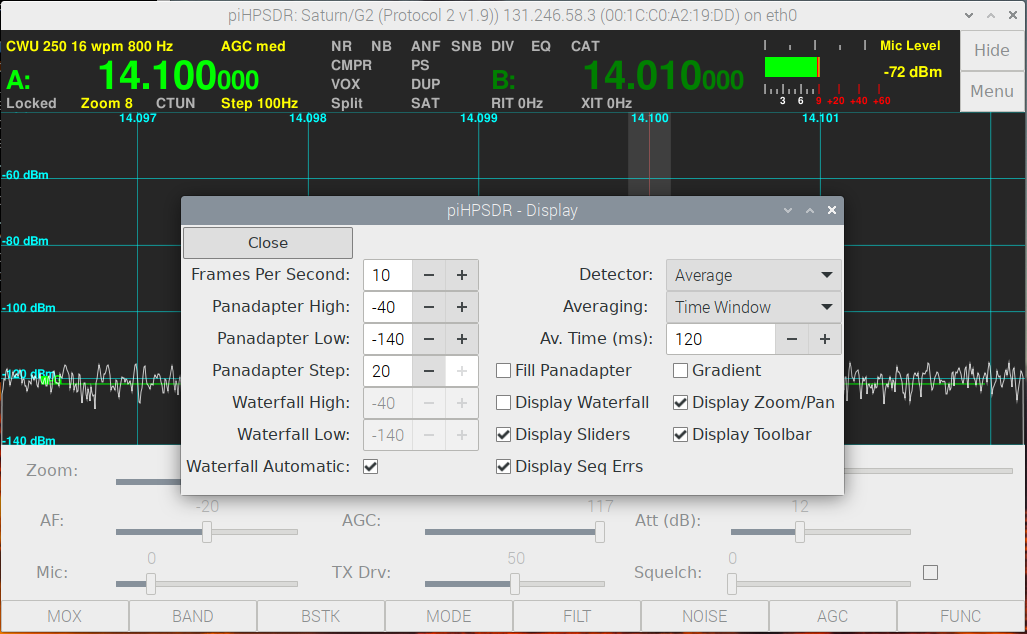
\includegraphics[width=12cm]{DisplayMenu.png}
\end{center}

\section{The \texttt{Meter} menu}
\begin{center}
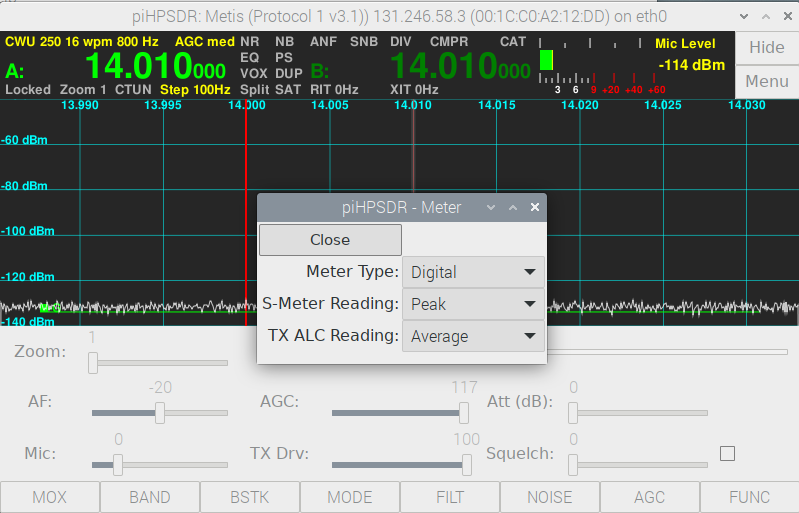
\includegraphics[width=12cm]{MeterMenu.png}
\end{center}

\section{The \texttt{XVTR} (Transverter) Menu}
\begin{center}
\includegraphics[width=12cm]{XVTRMenu.png}
\end{center}

\chapter{The Main Menu: VFO-related menus}

\section{The \texttt{FREQ} (VFO) menu}
\begin{center}
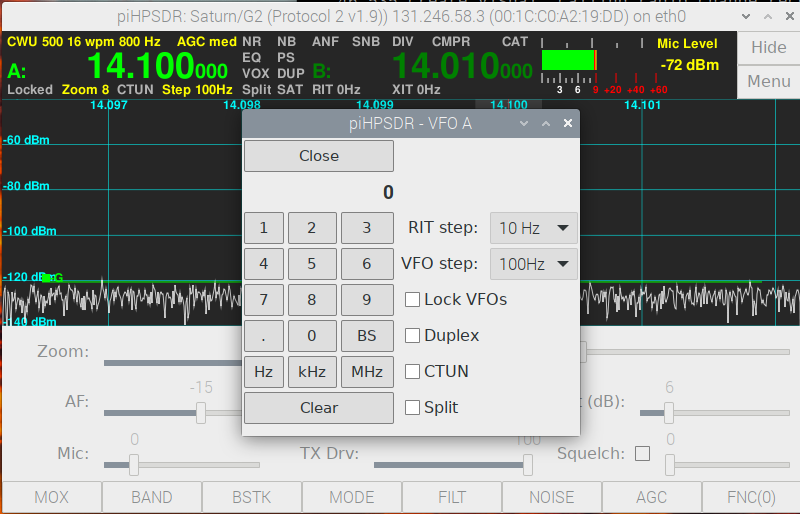
\includegraphics[width=12cm]{VFOmenu.png}
\end{center}

\section{The \texttt{Band} menu}
\begin{center}
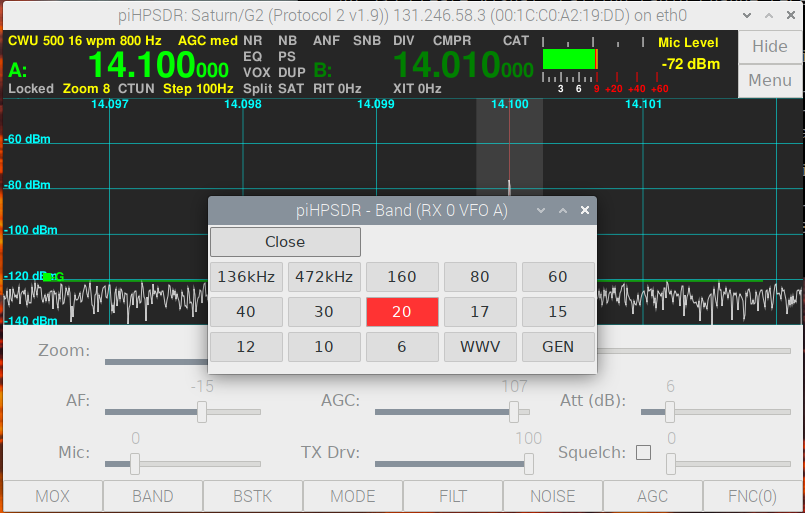
\includegraphics[width=12cm]{BandMenu.png}
\end{center}

\section{The  \texttt{BStack} (Bandstack) menu}
\begin{center}
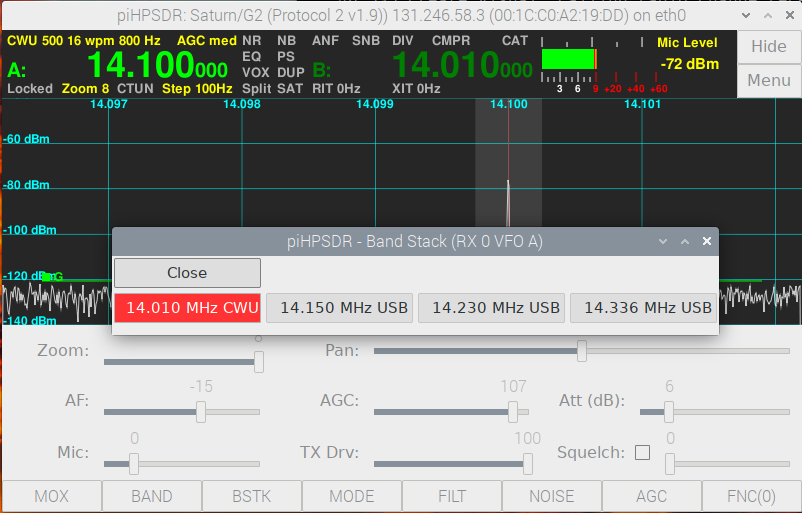
\includegraphics[width=12cm]{BandstackMenu.png}
\end{center}
 
\section{The \texttt{Mode} menu}
\begin{center}
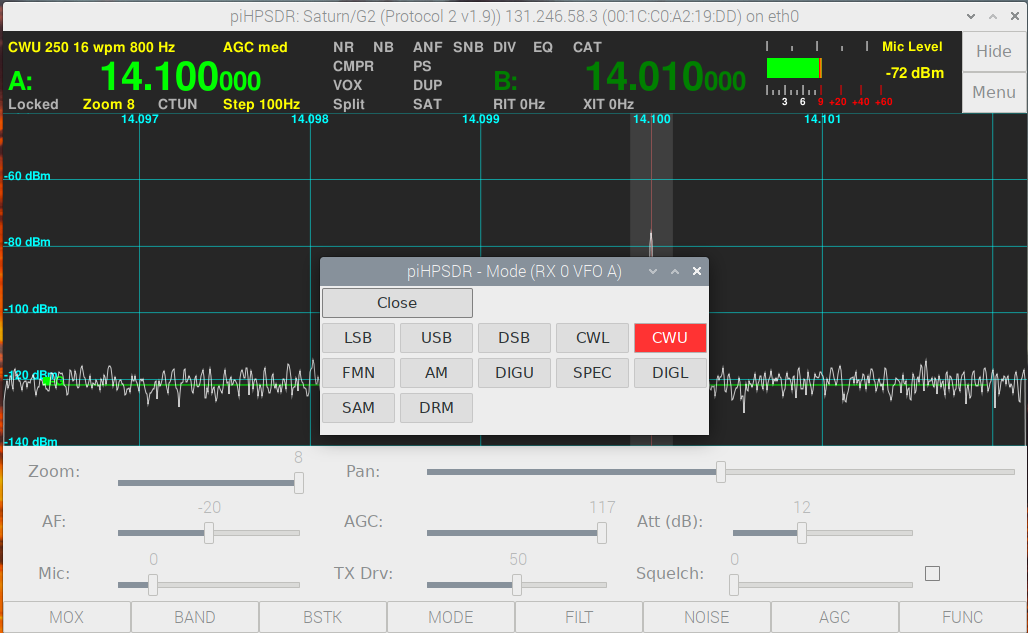
\includegraphics[width=12cm]{ModeMenu.png}
\end{center}

\section{The \texttt{MEM} (Memory) menu}
\begin{center}
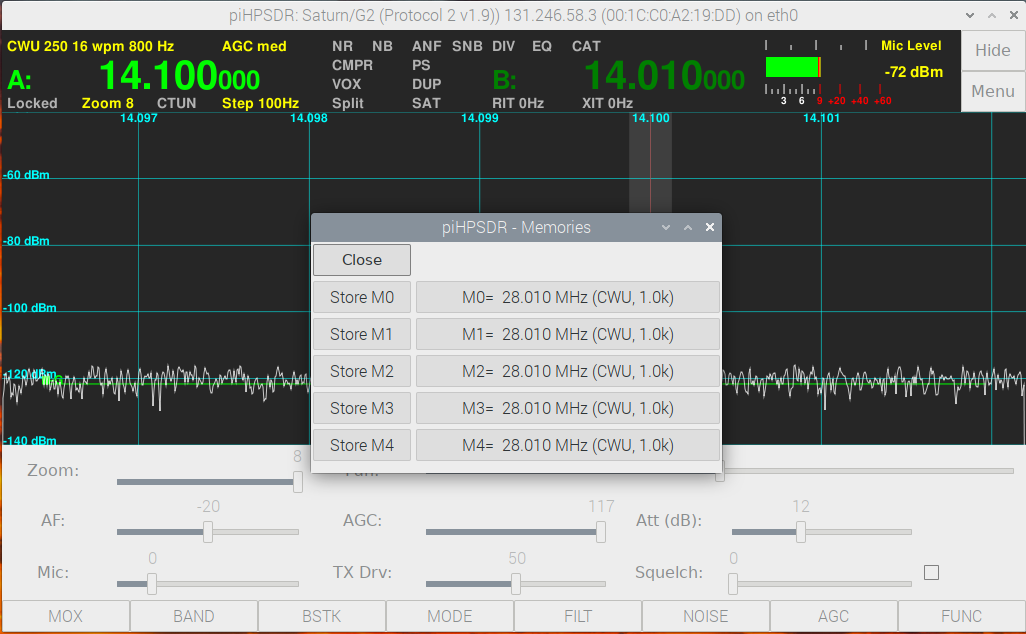
\includegraphics[width=12cm]{MemMenu.png}
\end{center}
 
\chapter{The Main Menu: RX-related menus}

\section{The \texttt{RX} Menu}
\begin{center}
\includegraphics[width=12cm]{RXMenu.png}
\end{center}

\section{The \texttt{Filter} menu}
\begin{center}
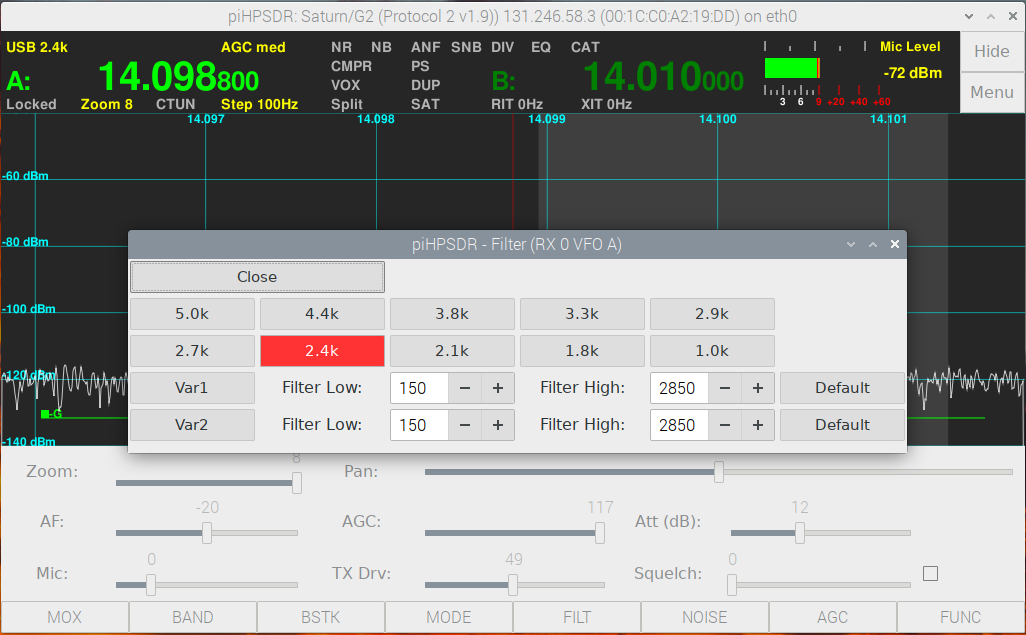
\includegraphics[width=12cm]{FilterMenuUSB.png}
\end{center}
\begin{center}
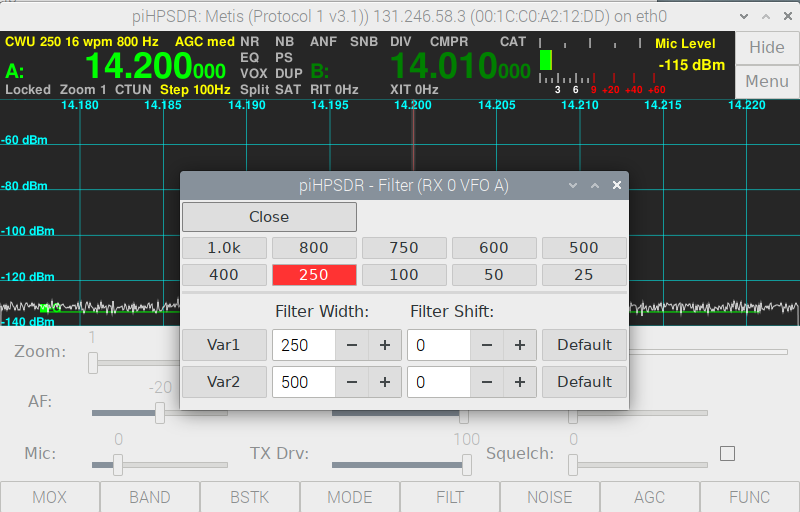
\includegraphics[width=12cm]{FilterMenuCW.png}
\end{center}
\section{The \texttt{Noise} Menu}
\begin{center}
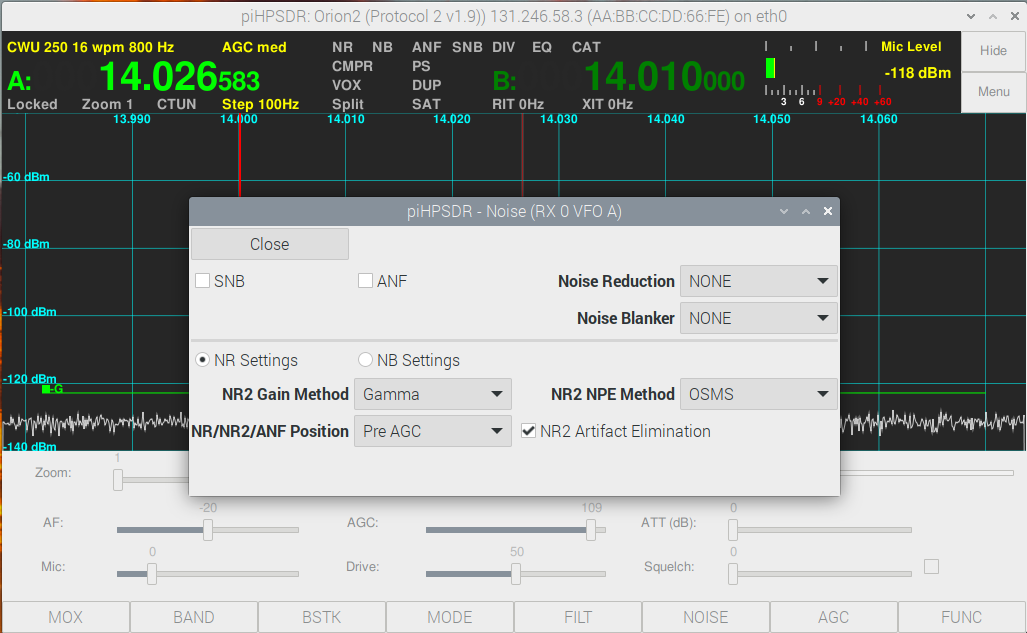
\includegraphics[width=12cm]{NoiseMenu1.png}
\end{center}

\begin{center}
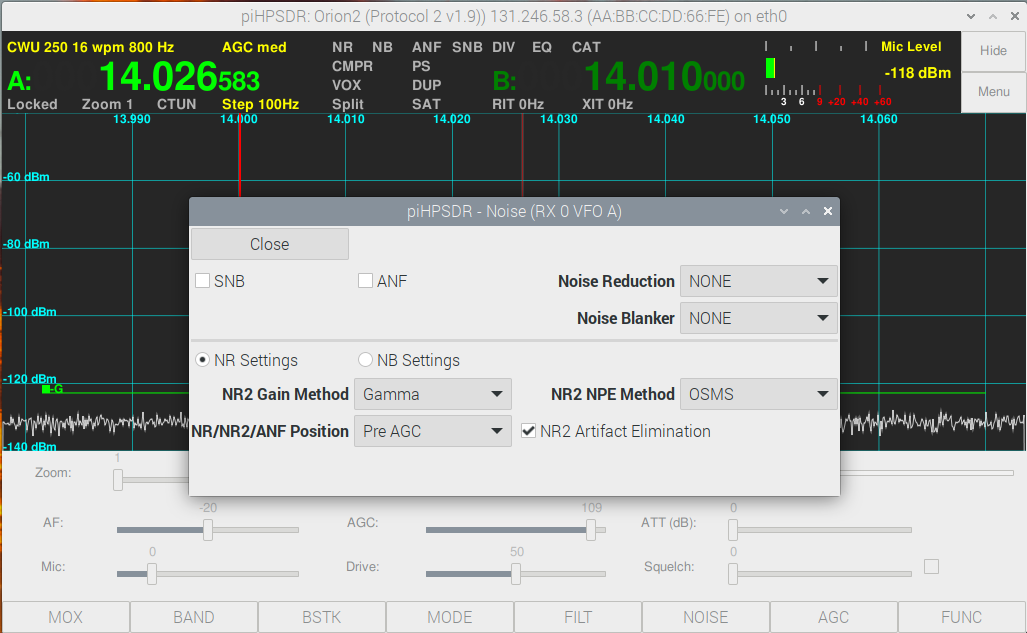
\includegraphics[width=12cm]{NoiseMenu1.png}
\end{center}

\section{The \texttt{AGC} Menu}
\begin{center}
\includegraphics[width=12cm]{AGCMenu.png}
\end{center}

\section{The \texttt{Diversity} Menu}
\begin{center}
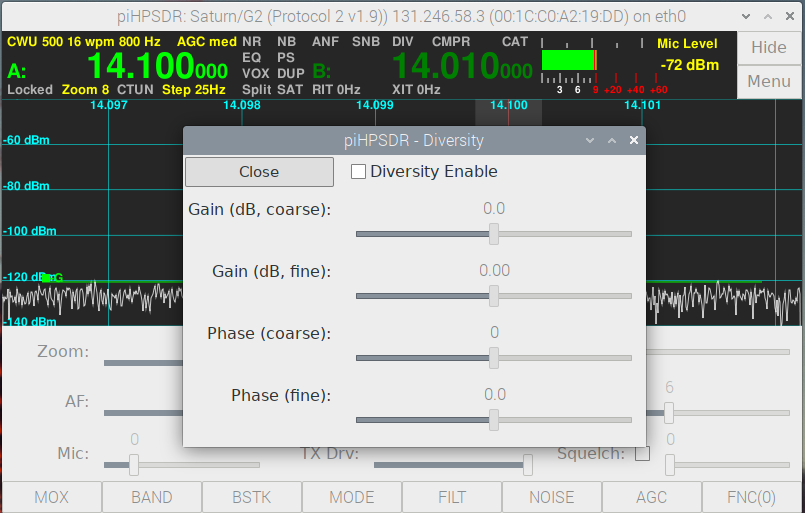
\includegraphics[width=12cm]{DiversityMenu.png}
\end{center}

\chapter{The Main Menu: TX-related menus}

\section{The \texttt{TX} Menu}
\begin{center}
\includegraphics[width=12cm]{TXMenu.png}
\end{center}

\section{The \texttt{PA} Menu}
\begin{center}
\includegraphics[width=12cm]{PAMenuCalibrate.png}
\end{center}

\begin{center}
\includegraphics[width=12cm]{PAMenuWatt.png}
\end{center}

\section{The \texttt{VOX} Menu}
\begin{center}
\includegraphics[width=12cm]{VOXMenu.png}
\end{center}

\section{The \texttt{PS} (PureSignal) Menu}
\begin{center}
\includegraphics[width=12cm]{PSMenu.png}
\end{center}
\begin{center}
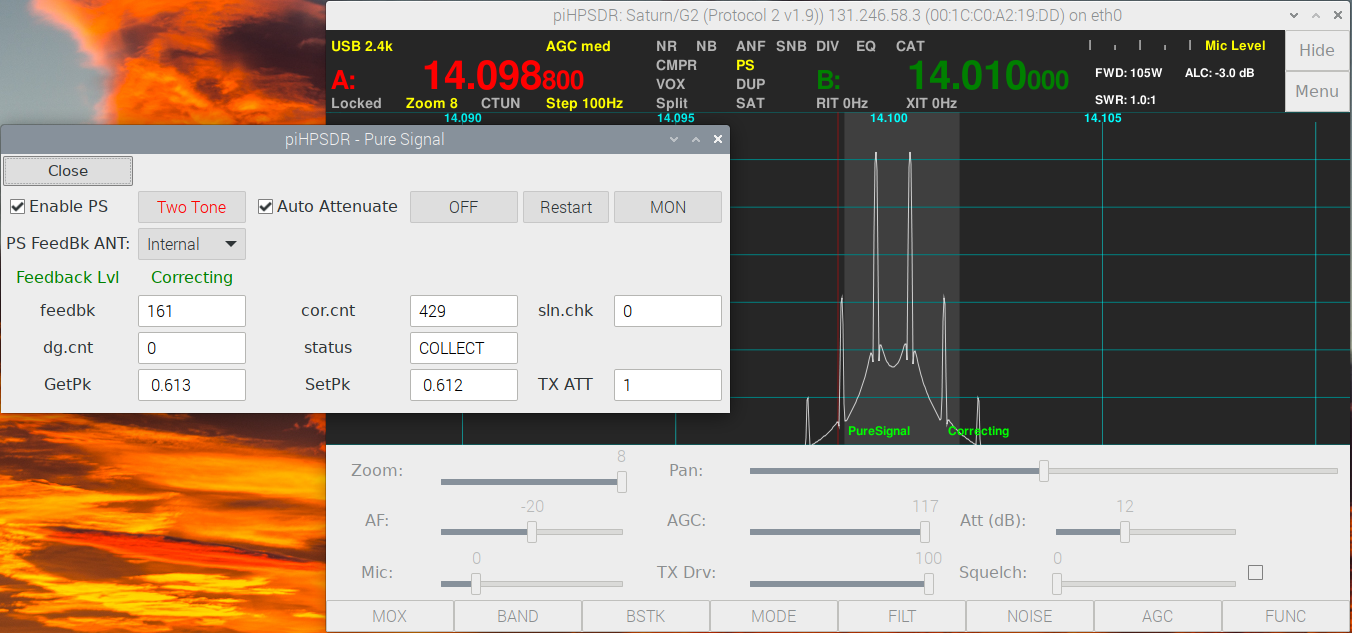
\includegraphics[width=12cm]{PSnomon.png}
\end{center}
\begin{center}
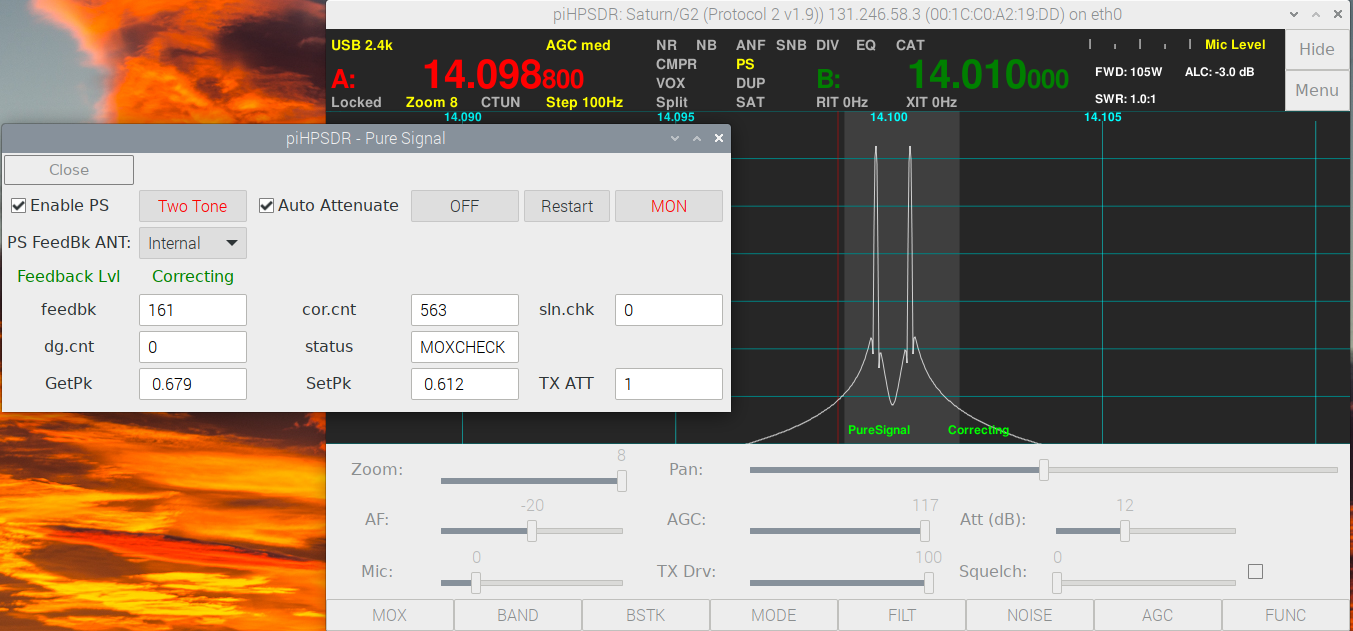
\includegraphics[width=12cm]{PSmon.png}
\end{center}
\begin{center}
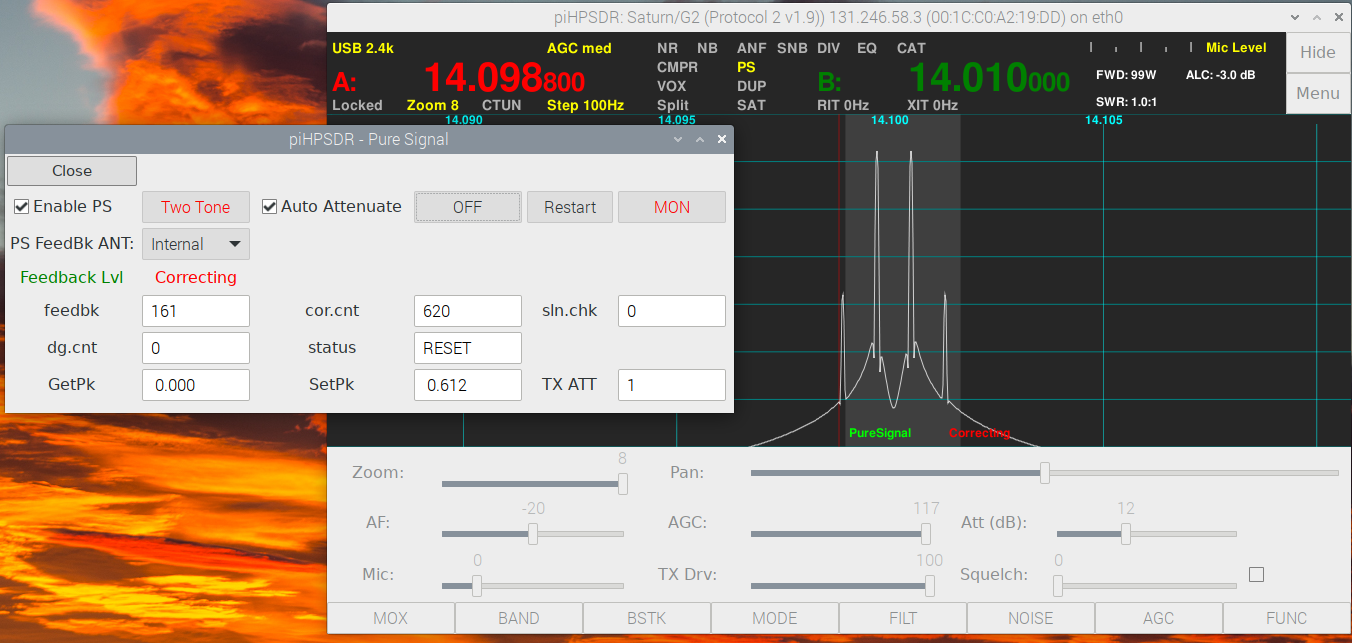
\includegraphics[width=12cm]{PSoff.png}
\end{center}

\section{The \texttt{CW} Menu}
\begin{center}
\includegraphics[width=12cm]{CWMenu.png}
\end{center}

\chapter{The Main Menu: menus for RX and TX}

\section{The \texttt{FFT} (Signal Processing) Menu}
\begin{center}
\includegraphics[width=12cm]{FFTMenu.png}
\end{center}

\section{The \texttt{Equalizer} Menu}
\begin{center}
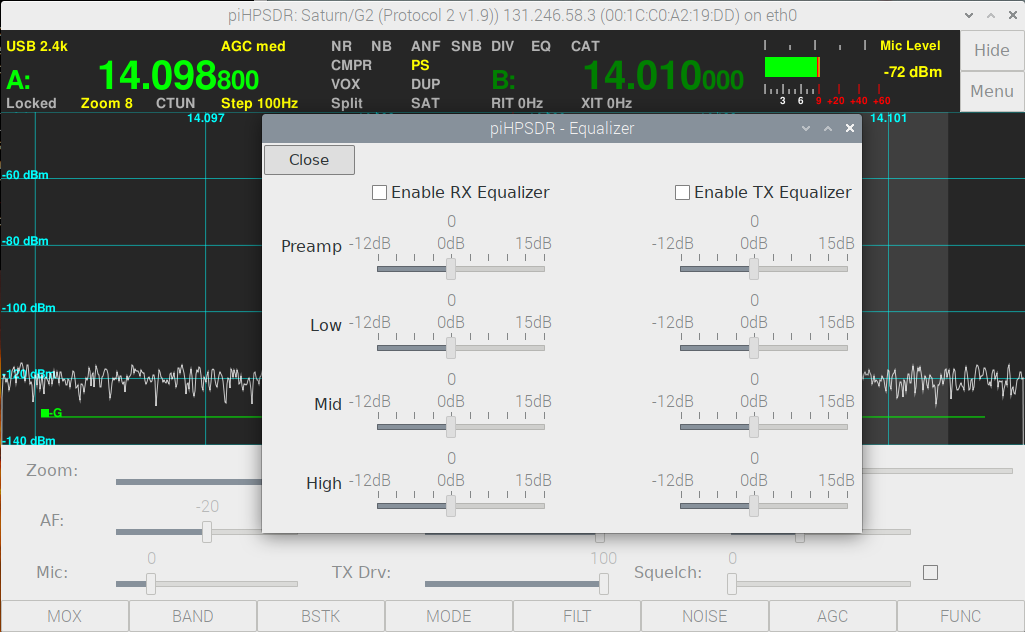
\includegraphics[width=12cm]{EqualizerMenu.png}
\end{center}

\section{The \texttt{Ant} (Antenna) Menu}
\begin{center}
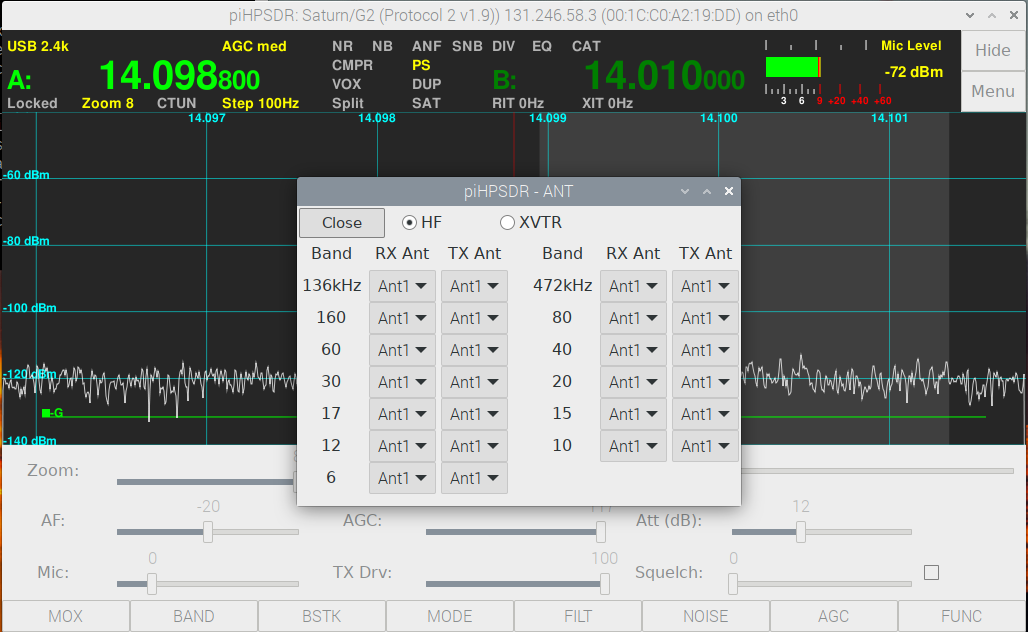
\includegraphics[width=12cm]{AntMenu.png}
\end{center}
 
\section{The \texttt{OC} (OpenCollector) Menu}
\begin{center}
\includegraphics[width=12cm]{OCMenu.png}
\end{center}

\chapter{The Main Menu: controlling piHPSDR}

In this chapter, the customization of the toolbar (at the bottom of the piHPSDR window),
as well as how to configure GPIO and MIDI controllers, is described. Furthermore, in this
chapter we discuss the RIGCTL menu which allows controlling piHPSDR by some external program
such as a logbook or contest program, via standardized CAT commands that can be sent to
piHPSDR either over a serial line or via TCP.

\textbf{Note for Controller1 owners:} The eight switches (push-buttons) of the controller,
that a positioned below the screen, are bound to the eight toolbar buttons on the screen.
Therefore, there is no "Switches" menu for this controller, and the switches are implicitly
configured via the Toolbar menu.

\section{The \texttt{Toolbar} Menu}
We start with the "Toolbar" menu, that can be found at the top of the rightmost
column in the main menu. The toolbar consists of eight buttons that can be assigned
to a set of eight functions. There are six such sets, and pressing the FUNC button
cycles through these six sets. If you click the Toolbar button, a menu pops up and
you see the following:

\begin{center}
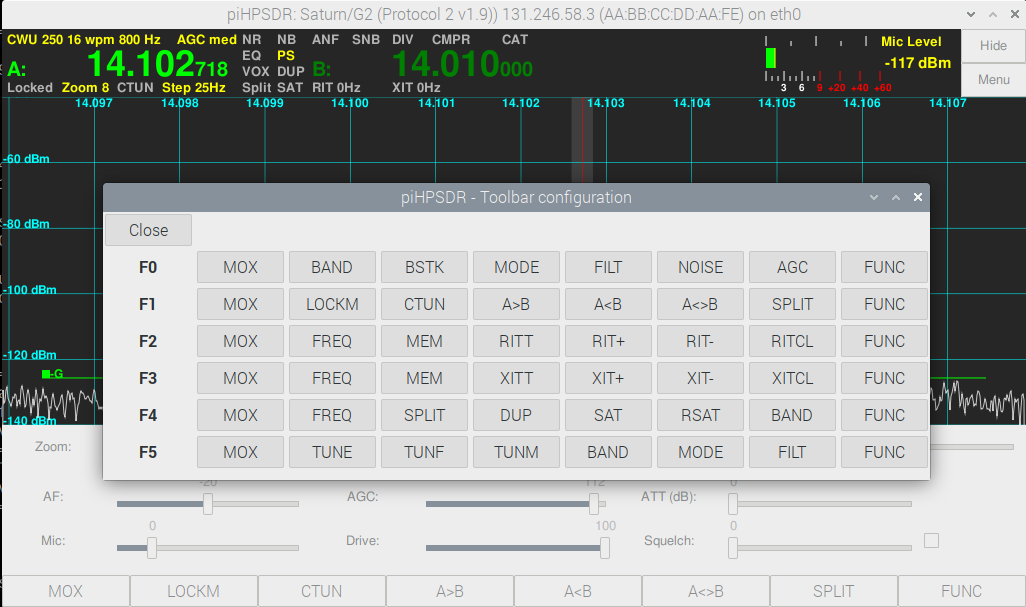
\includegraphics[width=12cm]{ToolbarMenu1.png}
\end{center}

The six lines denoted \texttt{F0} through \texttt{F5} indicate the six different sets. If you
look closely, you will discover that the set \texttt{F0} is the one that is currently active,
since the labels in this line exactly match the labels in the toolbar. In this menu, the
possible actions (that can be bound to a button) are written with the short text (see Appendix A),
since this is the text that is printed on the toolbar buttons. If one now clicks (just an example)
the \texttt{CTUN} button in the line \texttt{F1}, an ,,action dialog'' pops up that looks as follows:

\begin{center}
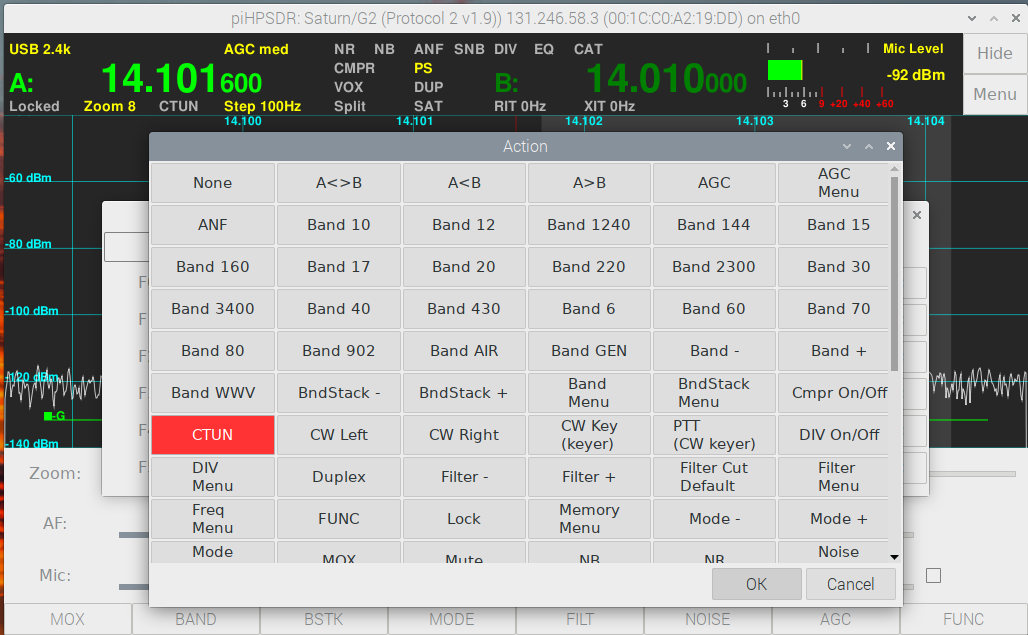
\includegraphics[width=12cm]{ToolbarMenu2.png}
\end{center}

The current action selected (\texttt{CTUN}) is high-lighted. Lists of possible actions can be rather long,
so it might be necessary that you have to scroll up or down in such an action dialog until you have
found what you were looking for. Now (again just an example) the button \texttt{Band 20} has been clicked
in the action dialog, such that it gets high-lighted:

\begin{center}
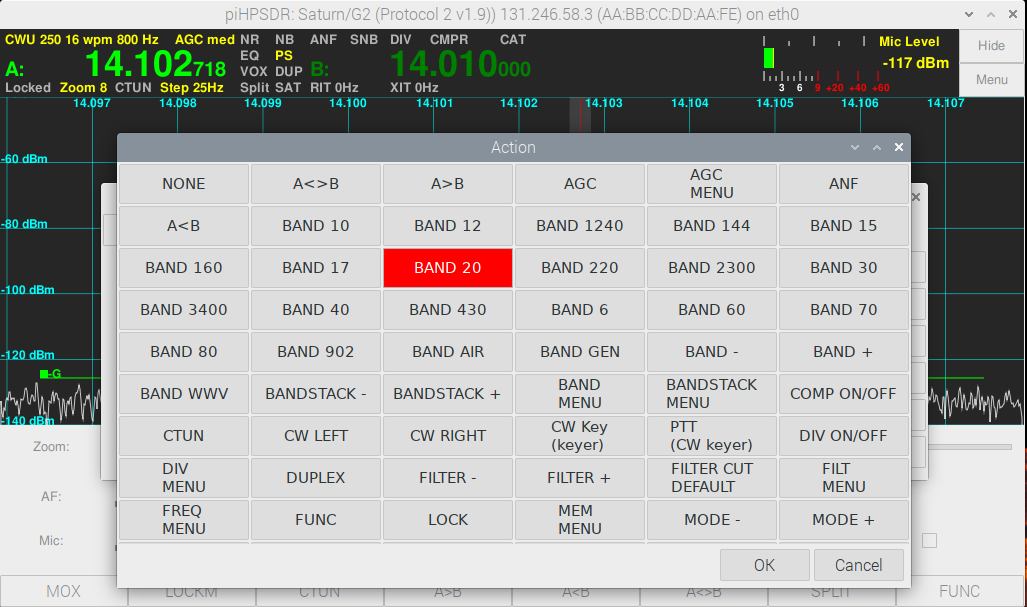
\includegraphics[width=12cm]{ToolbarMenu3.png}
\end{center}

If one now closes the action dialog by clicking the \texttt{OK} button, the third button in the \texttt{F1}
line of the toolbar menu has changed, it now gives the short text (\texttt{20}) of the action, which will
switch the active receiver to the 20m band (see the explanation of all the actions in Appendix A).

\begin{center}
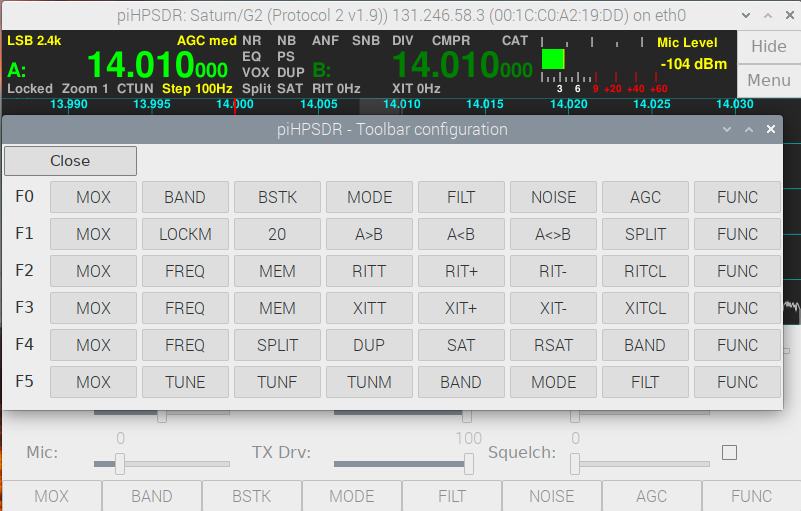
\includegraphics[width=12cm]{ToolbarMenu4.png}
\end{center}
You also see that the toolbar has not changed, because we have just changed the \texttt{F1} set,
while currently the \texttt{F0} set is active. If one now, however, clicks the \texttt{FUNC}
button at the bottom right one advances to the \texttt{F1} set and the toolbar labels
are updated: 

\begin{center}
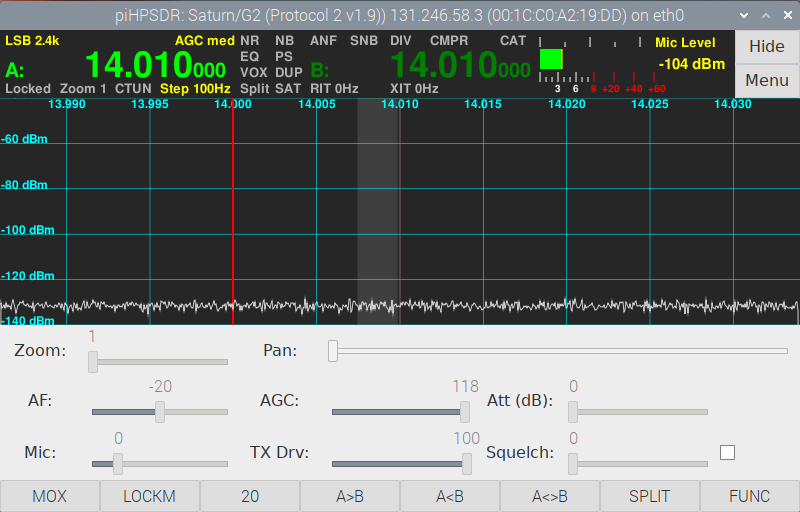
\includegraphics[width=12cm]{ToolbarMenu5.png}
\end{center}

Note that it is not possible to change the assignment of the  rightmost button of the toolbar,
it will always be assigned to \texttt{FUNC}, since if one has no access to this
function, one no longer cycle through the sets.


\section{The \texttt{RIGCTL} (CAT control) Menu}
\begin{center}
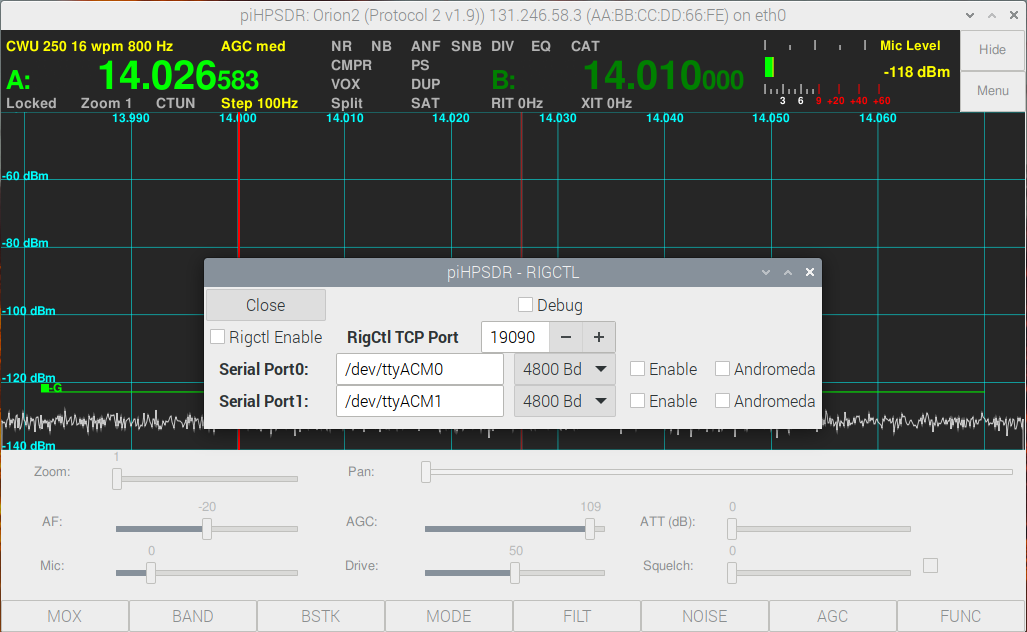
\includegraphics[width=12cm]{RigCtlMenu.png}
\end{center}

\section{The \texttt{MIDI} Menu}
\begin{center}
\includegraphics[width=12cm]{MIDImenu1.png}
\end{center}

\begin{center}
\includegraphics[width=12cm]{MIDImenu2.png}
\end{center}

\begin{center}
\includegraphics[width=12cm]{MIDImenu3.png}
\end{center}
 
\section{The \texttt{Encoders} Menu}
\begin{center}
\includegraphics[width=12cm]{EncoderMenuG2.png}
\end{center}

\begin{center}
\includegraphics[width=12cm]{EncoderMenuV2.png}
\end{center}

\begin{center}
\includegraphics[width=12cm]{EncoderMenuV1.png}
\end{center}


\section{The \texttt{Switches} Menu}
\begin{center}
\includegraphics[width=12cm]{SwitchMenuG2.png}
\end{center}

\begin{center}
\includegraphics[width=12cm]{SwitchMenuV2.png}
\end{center}

\appendix
\chapter{List of piHPSDR ,,Actions''}

In this chapter, we give a list of ,,actions'' implemented in the piHPSDR program. These actions can be assigned to
toolbar buttons on the screen, or pushbuttons/encoders of a GPIO-connected or MIDI controller. Not all actions can
be assigned to all control elements. Changing the AF volume, for example, can only be assigned to a knob which
you can turn, while switching RIT on/off can only be assigned to a button that you can push. For each action
in the following table, there is a long and a short string assigned. The long string will be used when there is
enough space, while the short string is used for small buttons and to store actions in preference files (therefore
the short strings never contain a blank character or a line break). Then, for each action we give the type of control
element allowed for this action as a combination of the letters B, P, E, which stand for

\begin{itemize}[font=\texttt, left=0pt]
\item[B] {"Button": A button in the toolbar, or a push-button or switch on a GPIO or MIDI connected console}
\item[P] {"Potentiometer": A potentiometer or a slider on a MIDI connected console}
\item[E] {"Encoder": A rotary encoder on a GPIO or MIDI connected console}
\end{itemize}

The main difference between a "potentiometer" and an "encoder" is, that the former has a min and max position, while
an encoder can be turned in either direction without stopping. This means that a potentiometer
reports a value between min and max, while an encoder reports an increment,
that is, whether it has been turned clock wise or counter clock wise.
The existing GPIO consoles do not have potentiometers (most likely because of the lack of analog inputs), but
many MIDI consoles do have, and Arduino-based MIDI controllers might have it because there analog inputs
to read out potentiometers are available.

To give an example, controlling the TX drive can be down both with a slider and with an encoder. While for
a slider/potentiometer, the values from min to max are simple mapped to the TX drive values from 0 to 100,
the signals from an encoder will just increase or decrease the value until one of a limits has been reached.

In the following, the actions are alphabetically sorted by their long name, with the "empty" action listed
first.

\renewcommand{\belowrulesep}{0pt}
\renewcommand{\aboverulesep}{0pt}
\def\action#1#2#3#4{
\begin{center}
\begin{tabular}{|p{5cm}|p{5cm}|p{1cm}|}
\toprule
$\phantom{\Big|}$\texttt{\large #1} & \texttt{\large #2} & \texttt{\large #3} \\\cline{1-3}
\multicolumn{3}{|p{\textwidth}|}{#4} \\
\bottomrule
\end{tabular}
\end{center}
}


\action{NONE}{NONE}{BPE}{This is an action which does nothing. It can be assigned to buttons or enco\-ders that
are often accidentally operated. Some MIDI consoles, for example, report a button press event if the VFO
knob is touched, and this we want to ignore.}

\action{A<>B}{A<>B}{B}{Swap VFOs A and B. This will not only swap the frequencies, but also all other settings
associated with that VFO, such as mode, filter, CTUN, and RIT settings.}

\action{A<B}{A<B}{B}{Copy VFO B to VFO A.}

\action{A>B}{A>B}{B}{Copy VFO A to VFO B.}

\action{AF GAIN}{AFGAIN}{PE}{Change the AF gain (headphone volume) of the active receiver.}

\action{AF GAIN RX1}{AFGAIN1}{PE}{Change the AF gain (headphone volume) of the RX1 receiver.}

\action{AF GAIN RX2}{AFGAIN2}{PE}{Change the AF gain (headphone volume) of the RX2 receiver.}

\action{AGC MENU}{AGC}{B}{Opens the \texttt{AGC} menu.}

\action{ANF}{ANF}{B}{Toggels the state (on/off) of the automatic notch filter for the active receiver.}

\action{ATTEN}{ATTEN}{PE}{Changes the value (0-31 dB) of the step attenuator of the active receiver.
This funciton is only available for radios that have such an attenuator.}

\action{BAND 10}{10}{B}
{Change band of the active receiver to the 10m band. If already on that band, move to
the next bandstack entry. This action is a no-op if the frequency of the band falls outside the frequency range
of the radio.} 

\action{BAND 12}{12}{B}
{Change band of the active receiver to the 12m band. If already on that band, move to
the next bandstack entry. This action is a no-op if the frequency of the band falls outside the frequency range
of the radio.}

\action{BAND 1240}{1240}{B}
{Change band of the active receiver to the 1240 MHz (23 cm) band. If already on that band, move to
the next bandstack entry. This action is a no-op if the frequency of the band falls outside the frequency range
of the radio.}

\action{BAND 144}{144}{B}
{Change band of the active receiver to the 144 MHz (2m) band. If already on that band, move to
the next bandstack entry. This action is a no-op if the frequency of the band falls outside the frequency range
of the radio.}

\action{BAND 15}{15}{B}
{Change band of the active receiver to the 15m band. If already on that band, move to
the next bandstack entry. This action is a no-op if the frequency of the band falls outside the frequency range
of the radio.}

\action{BAND 160}{160}{B}
{Change band of the active receiver to the 160m band. If already on that band, move to
the next bandstack entry. This action is a no-op if the frequency of the band falls outside the frequency range
of the radio.}

\action{BAND 17}{17}{B}
{Change band of the active receiver to the 15m band. If already on that band, move to
the next bandstack entry. This action is a no-op if the frequency of the band falls outside the frequency range
of the radio.}

\action{BAND 20}{20}{B}
{Change band of the active receiver to the 15m band. If already on that band, move to
the next bandstack entry. This action is a no-op if the frequency of the band falls outside the frequency range
of the radio.}

\action{BAND 220}{220}{B}
{Change band of the active receiver to the 220 MHz (1.25 m) band. If already on that band, move to
the next bandstack entry. This action is a no-op if the frequency of the band falls outside the frequency range
of the radio.}

\action{BAND 2300}{2300}{B}
{Change band of the active receiver to the 2300MHz (13 cm) band. If already on that band, move to
the next bandstack entry. This action is a no-op if the frequency of the band falls outside the frequency range
of the radio.}

\action{BAND 30}{30}{B}
{Change band of the active receiver to the 30m band. If already on that band, move to
the next bandstack entry. This action is a no-op if the frequency of the band falls outside the frequency range
of the radio.}

\action{BAND 3400}{3400}{B}
{Change band of the active receiver to the 3400 Mhz (9 cm) band. If already on that band, move to
the next bandstack entry. This action is a no-op if the frequency of the band falls outside the frequency range
of the radio.}

\action{BAND 40}{40}{B}
{Change band of the active receiver to the 40m band. If already on that band, move to
the next bandstack entry. This action is a no-op if the frequency of the band falls outside the frequency range
of the radio.}

\action{BAND 430}{430}{B}
{Change band of the active receiver to the 430 MHz (70 cm) band. If already on that band, move to
the next bandstack entry. This action is a no-op if the frequency of the band falls outside the frequency range
of the radio.}

\action{BAND 6}{6}{B}
{Change band of the active receiver to the 6m band. If already on that band, move to
the next bandstack entry. This action is a no-op if the frequency of the band falls outside the frequency range
of the radio.}

\action{BAND 60}{60}{B}
{Change band of the active receiver to the 60m band. If already on that band, move to
the next bandstack entry. This action is a no-op if the frequency of the band falls outside the frequency range
of the radio.}

\action{BAND 70}{70}{B}
{Change band of the active receiver to the 70 MHz (4m)  band. If already on that band, move to
the next bandstack entry. This action is a no-op if the frequency of the band falls outside the frequency range
of the radio.}

\action{BAND 80}{80}{B}
{Change band of the active receiver to the 80m band. If already on that band, move to
the next bandstack entry. This action is a no-op if the frequency of the band falls outside the frequency range
of the radio.}

\action{BAND 902}{902}{B}
{Change band of the active receiver to the 902 MHz (33 cm) band. If already on that band, move to
the next bandstack entry. This action is a no-op if the frequency of the band falls outside the frequency range
of the radio.}

\action{BAND AIR}{AIR}{B}
{Change band of the active receiver to the 108 MHz band, used for aircraft communication. If already on that band, move to
the next bandstack entry. This action is a no-op if the frequency of the band falls outside the frequency range
of the radio.} 

\action{BAND GEN}{GEN}{B}
{Change band of the active receiver to the current bandstack entry of the "general" band. If already on that band, move to
the next bandstack entry. This action is a no-op if the frequency of the band falls outside the frequency range
of the radio.}

\action{BAND -}{BND-}{B}
{Change band of the active receiver to the next lower band in the list of bands. If already at the lowest band, switch to
the highest band (including transverter bands which have been defined) whose frequency is with the radio's frequency range.}

\action{BAND +}{BND+}{B}
{Change band of the active receiver to the next higher band in the list of bands (including transverter bands that have been
defined). If already at the highest band, switch to
the lowest band whose frequency is with the radio's frequency range.}

\action{BAND WWV}{WWV}{B}
{Change band of the active receiver to the current bandstack entry of the WWV band. If already on that band, move to
the next bandstack entry. This action is a no-op if the frequency of the band falls outside the frequency range
of the radio.}

\action{BANDSTACK -}{BSTK-}{B}
{Cylcle backward through the bandstack entries of the active receiver.}

\action{BANDSTACK +}{BSTK+}{B}
{Cylcle forward through the bandstack entries of the active receiver.}

\action{BAND MENU}{BAND}{B}
{Open the \texttt{BAND} menu.}

\action{BANDSTACK MENU}{BSTK}{B}
{Open the \texttt{BANDSTACK} menu.}

\action{COMP ON/OFF}{COMP}{B}
{Toggle the state (on/off) of the compressor used in the TX audio input.}

\action{COMPRESSION}{COMPVAL}{PE}
{Change the value of the compressor (0-20 dB) used in the TX audio input. The compressor is automaticall switched on (off) if
the "new" value of the compressor is larger then  (equal to) zero.}

\action{CTUN}{CTUN}{B}
{Toggle the state (on/off) of the CTUN state of the active receiver. CTUN stands for "click to tune". In CTUN mode, you can move
the RX frequency over the whole spectrum scope, whose center then remains at a fixed frequency.}

\action{CW FREQUENCY}{CWFREQ}{PE}
{Change the CW side tone frequency in the range 300-1000 Hz. This also changes the BFO frequency upon receive.}

\action{CW LEFT}{CWL}{B}
{This action indicates the closure/opening of the left paddle of a CW key. It is usually assigned to a GPIO line or a MIDI
controller to which a Morse paddle is attached, and works with the iambic keyer that is built into piHPSDR. This keyer
is only active if CW is \textit{not} handled in the radio (see CW menu).}

\action{CW RIGHT}{CWR}{B}
{This action indicates the closure/opening of the right paddle of a CW key. It is usually assigned to a GPIO line or a MIDI
controller to which a Morse paddle is attached, and works with the iambic keyer that is built into piHPSDR. This keyer
is only active if CW is \textit{not} handled in the radio (see CW menu).}

\action{CW SPEED}{CWSPD}{PE}
{Change the CW side tone frequency in the range 1-60 wpm. This affect the built-in iambic keyer or the keyer inside the radio,
depending on whether CW is handled in the radio or not (see CW menu).}

\action{CW Key (keyer)}{CWKy}{B}{Straith key key-down or key-up event. Usually assigned to a GPIO line of  MIDI controller to
which a straight key or an external keyer is attached. Note that this action does not automatically switch to TX, so it must
be used together with either manual RX/TX switching, or with the "\texttt{PTT (CW Keyer)}" action.}

\action{PTT (keyer)}{CWKyPTT}{B}{This very similar to the \texttt{PTT} action (see below) with the exception that CW handling
in the radio is temporarily disabled (thus, CW handling in piHPSDR is enabled). This allows to have, e.g. a paddle attached
to the radio while a contest logging program ,,talks'' to piHPSDR.}

\action{DIV ON/OFF}{DIVT}{B}{Toggles (enabled/disabled) DIVERSITY reception.}

\action{DIV GAIN}{DIVG}{E}{Adjust DIVERSITY gain. One tick of the encoder increments of decrements the gain by an amount of 0.5}

\action{DIV GAIN COARSE}{DIVGC}{E}{Adjust DIVERSITY gain (coarse adjustment).  One tick of the encoder increments of decrements the gain by an amount of 2.5}

\action{DIV GAIN FINE}{DIVGF}{E}{Adjust DIVERSITY gain (fine adjustment).  One tick of the encoder increments of decrements the gain by an amount of 0.1.
Since adjusting the DIVERSITY gain (or phase) is sometimes difficult, assigning one encoder to a coarse and another encoder to a fine adjustment may
help in locating the ,,sweet spot''.}

\action{DIV PHASE}{DIVP}{E}{Adjust DIVERSITY phase (fine adjustment). One tick of the encoder increments of decrements the gain by an amount of 0.5}

\action{DIV PHASE COARSE}{DIVPC}{E}{Adjust DIVERSITY gain (coarse adjustment). One tick of the encoder increments of decrements the gain by an amount of 2.5}

\action{DIV PHASE FINE}{DIVPF}{E}{Adjust DIVERSITY gain (coarse adjustment). One tick of the encoder increments of decrements the gain by an amount of 20.1}

\action{DIV MENU}{DIV}{B}{Open the DIVERSITY menu.}

\action{DUPLEX}{DUP}{B}{Toggle (on/off) DUPLEX status. IN the DUPLEX mode, the receivers continue to work during TX, and the RX panels are not
removed during TX. Instead, a separate TX window opens during transmitting. Generally, DUPLEX only make sense when using different and well
decoupled RX and TX antennas.}

\action{FILTER -}{FL-}{B}{Cycle forward (!) through the list of filters for the current mode of the active receiver. Normally, this means switching
to a narrower filter (hence the name \texttt{FILTER -}). When reaching the last filter in the list, further cycling switches to the first
(widest) filter.}

 \action{FILTER +}{FL+}{B}{Cycle backward (!) through the list of filters for the current mode of the active receiver. Normally, this means switching
to a wider filter (hence the name \texttt{FILTER +}). When reaching the first filter in the list, further cycling switches to the last
filter which is the variable \texttt{Var2} filter.}

\action{FILTER CUT LOW}{FCUTL}{E}{Adjust the low-cut of the current filter. Note that the notion of ,,low'' edge of the filter refers to
audio frequencies for the single side band modes LSB, CWL, DIGL. This action is a no-op unless the current filter is one of the two variable filters
 \texttt{Var1} or \texttt{Var2}.}

\action{FILTER CUT HIGH}{FCUTL}{E}{Adjust the high-cut of the current filter. Note that the notion of ,,high'' edge of the filter refers to
audio frequencies for the single side band modes LSB, CWL, DIGL. This action is a no-op unless the current filter is one of the two variable filters
 \texttt{Var1} or \texttt{Var2}.}
 
 \action{FILTER CUT DEFAULT}{FCUTDEF}{B}{Reset the low and high cut of the current filter to the default values. This action is a no-op unless the current filter is one of the two variable filters
 \texttt{Var1} or \texttt{Var2}.}
 
 \action{FILT MENU}{FILT}{B}{This opens the \texttt{Filter} menu.}
 
 \action{FREQ MENU}{FREQ}{B}{This opens the \texttt{FREQ} (VFO) menu.}
 
 \action{FUNC}{FUNC}{B}{Cycle through the six toolbar sets. For the piHPSDR GPIO controller V1, where the eight switches follow the toolbar buttons, this also affects the function
 of the switches. Note that this action is \textit{always} connected with the right-most toolbar button.}
 
 \action{IF SHIFT}{IFSHFT}{E}{This command is effective only if one of the variable filters Var1 or Var2 is currently used in the  active receiver, and shifts the  filter, that is,
 it affects  the low and high cut in the same way.}
 
 \action{IF SHIFT RX1}{IFSHFT1}{E}{This command is effective only if one of the variable filters Var1 or Var2 is currently used in VFO-A, and shifts the filter, that is,
 it affects  the low and high cut in the same way.}
 
 \action{IF SHIFT RX2}{IFSHFT2}{E}{This command is effective only if one of the variable filters Var1 or Var2 is currently used in VFO-B, and shifts the filter, that is,
 it affects  the low and high cut in the same way.}
 
 \action{IF WIDTH}{IFWIDTH}{E}{This command is effective only if one of the variable filters Var1 or Var2 is currently used in the  active receiver, and changes the  filter width, that is,
 it affects  the low and high cut in an opposite way.}
 
 \action{IF WIDTH RX1}{IFWIDTH1}{E}{This command is effective only if one of the variable filters Var1 or Var2 is currently used in VFO-A, and changes the  filter width, that is,
 it affects  the low and high cut in an opposite way.}
 
 action{IF WIDTH RX2}{IFWIDTH2}{E}{This command is effective only if one of the variable filters Var1 or Var2 is currently used in VFO-B, and changes the  filter width, that is,
 it affects  the low and high cut in an opposite way.}
 
\action{LINEIN GAIN}{LIGAIN}{PE}{Change the line-in gain of the radio. If the
     radio does not have a line-in input, this control has no effect.}
     
\action{LOCK}{LOCK}{B}{Lock the VFOs. A locked VFO will not accept VFO frequency steps in either direction, and cannot be moved by dragging with the  mouse. Band changes etc.
are still possible, though. The command is intended to guard against accidentally moving the VFO dial.}
  
\action{MEM MENU}{MEM}{B}{Open the \texttt{MEM} (Memory) menu.}
  
\action{MIC GAIN}{MICGAIN}{PE}{Change the mic gain (from -12 to 50 dB). The amplification of the microphone audio data is done in software, and applies to the TX audio
input samples whereever they come from. (See the discussion of local microphones in the \texttt{TX} menu.}

\action{MODE -}{MD-}{B}{Cycle backwards through the list of modes for the active receiver. When the first mode (LSB) has been reached, jump to the last one (DRM). Note that when
changing the mode, the current filter, noise reduction, equalizer, VFO step size, and TX compressor settings are stored for the old mode, and the settings last used with the
new mode are restored. This allows to quickly switch between SSB and CW, or between SSB and digi modes, without re-adjusting these settings.}

\action{MODE +}{MD+}{B}{Cycle forward through the list of modes for the active receiver. When the last mode (DRM) has been reached, jump to the first one (LSB). Note that when
changing the mode, the current filter, noise reduction, equalizer, VFO step size, and TX compressor settings are stored for the old mode, and the settings last used with the
new mode are restored. This allows to quickly switch between SSB and CW, or between SSB and digi modes, without re-adjusting these settings.}

\action{MOX}{MOX}{B}{Toggle between TX and RX. Unlike the PTT action, which puts the radio into TX when pressed and into RX when released, this button toggles the PTT state
when pressed.}

\action{MUTE}{MUTE}{B}{Toggles the ,,mute'' state of the active receiver. If a receiver is muted, it produces zero-amplitude audio output.}

\action{NB}{NB}{B}{Cycles through the noise blanker states (NB off/NB1/NB2).}

\action{NR}{NR}{B}{Cycles through the noise reduction states (NR off/NR1/NR2).}

\action{NOISE MENU}{NOISE}{B}{Opens the \texttt{NOISE} menu.}

\action{NUMPAD 0}{0}{B}{Used for direct frequency entry. This is the same as hitting the corresponding button ,,0''
in the \texttt{FREQ} (VFO) menu.}

\action{NUMPAD 1}{1}{B}{Used for direct frequency entry. This is the same as hitting the corresponding button ,,1''
in the \texttt{FREQ} (VFO) menu.}

\action{NUMPAD 2}{2}{B}{Used for direct frequency entry. This is the same as hitting the corresponding button ,,2''
in the \texttt{FREQ} (VFO) menu.}

\action{NUMPAD 3}{3}{B}{Used for direct frequency entry. This is the same as hitting the corresponding button ,,3''
in the \texttt{FREQ} (VFO) menu.}

\action{NUMPAD 4}{4}{B}{Used for direct frequency entry. This is the same as hitting the corresponding button ,,4''
in the \texttt{FREQ} (VFO) menu.}

\action{NUMPAD 5}{5}{B}{Used for direct frequency entry. This is the same as hitting the corresponding button ,,5''
in the \texttt{FREQ} (VFO) menu.}

\action{NUMPAD 6}{6}{B}{Used for direct frequency entry. This is the same as hitting the corresponding button ,,6''
in the \texttt{FREQ} (VFO) menu.}

\action{NUMPAD 7}{7}{B}{Used for direct frequency entry. This is the same as hitting the corresponding button ,,7''
in the \texttt{FREQ} (VFO) menu.}

\action{NUMPAD 8}{8}{B}{(Used for direct frequency entry. This is the same as hitting the corresponding button ,,8''
in the \texttt{FREQ} (VFO) menu.}

\action{NUMPAD 9}{9}{B}{Used for direct frequency entry. This is the same as hitting the corresponding button ,,9''
in the \texttt{FREQ} (VFO) menu.}

\action{NUMPAD BS}{BS}{B}{Used for direct frequency entry (BS = backstep). This is the same as hitting the corresponding button 
in the \texttt{FREQ} (VFO) menu. It cancels the last-entered digit.}

\action{NUMPAD CL}{CL}{B}{Used for direct frequency entry (CL = clear). This is the same as hitting the corresponding button 
in the \texttt{FREQ} (VFO) menu. It cancels all entered digits so far.}

\action{NUMPAD DEC}{DEC}{B}{Used for direct frequency entry (DEC = decimal point). This is the same as hitting the corresponding button 
in the \texttt{FREQ} (VFO) menu.}

\action{NUMPAD KHZ}{KHZ}{B}{Used for direct frequency entry. This is the same as hitting the corresponding button 
in the \texttt{FREQ} (VFO) menu. The VFO frequency is changed to the value entered so far, multiplied with 1,000. For example, to
go to 7.040 MHz, one can enter the sequence ,,7'', ,,0'', ,,4'', ,,0'', ,,KHZ''.}

\action{NUMPAD MHZ}{MHZ}{B}{Used for direct frequency entry. This is the same as hitting the corresponding button 
in the \texttt{FREQ} (VFO) menu. The VFO frequency is changed to the value entered so far, multiplied with 1,000,000.
For example, to go to 7.040 MHz, one can enter the sequence ,,7'', ,,DEC'', ,,0'', ,,4'', ,,MHZ''.}

\action{NUMPAD ENTER}{EN}{B}{Used for direct frequency entry. This is the same as hitting the corresponding button 
in the \texttt{FREQ} (VFO) menu. The VFO frequency is changed to the value entered so far.
For example, to go to 7.040 MHz, one can enter the sequence ,,7'',  ,,0'', ,,4'', ,,0'', ,,0'', ,,0'', ,,0''. This
is rarely used but offers Hz-resolution for the direct frequency entry.}

\action{PAN}{PAN}{E}{Change the PAN value. This control is only effective when the Zoom value is larger than 1.}

\action{PAN -}{PAN-}{B}{Decrease the PAN value by 100. This control is only effective when the Zoom value is larger than 1.}

\action{PAN +}{PAN+}{B}{Increase the PAN value by 100. This control is only effective when the Zoom value is larger than 1.}

\action{PAH HIGH}{PANH}{PE}{Change the dBm value (from -60 to +20) at the top of the spectrum scope of the active receiver. Values outside
this range can be set in the \texttt{DISPLAY} menu.}

\action{PAH LOW}{PANL}{PE}{Change the dBm value (from -160 to -60) at the bottom of the spectrum scope of the active receiver.
Values outside this range can be set in the \texttt{DISPLAY} menu.}

\action{PAN STEP}{PANS}{PE}{Change the step size (from 5 to 30) of the panadapter of the active receiver. This is the spacing
of the thin horizontal  lines in the spectrum scope.}

\action{PREAMP ON/OFF}{PRE}{B}{Toggle the preamp of the active receiver. Although the preamp switching is part of the HPSDR protocol,
this has no effect in current radio models since the preamp is hard-wired ,,on''.}

\action{PS ON/OFF}{PST}{B}{Toggle (on/off) adaptive predistortion (PureSignal).}

\action{PS MENU}{PS}{B}{Open the \texttt{PS} (PureSignal) menu.}

\action{PTT}{PTT}{B}{Put the radio  into TX mode when the button is pressed, and go back to RX when the button is released. This is
one of the few actions where a button release event is significant. When attaching, say, the PTT contact of a microphone to
a GPIO line for this purpose, take care of proper debouncine, since piHPSDR is not good at debouncing switches where both
the press and release events are significant.}

\action{RF GAIN}{RFGAIN}{PE}{Set the gain of the RF front end of the active receiver. Only effective for radios that have such a
gain control. Most HPSDR radios do not have RF  gain, they have a step attenuator in the RF front end instead. Small SDR radios
using the AD9866 chip (HermesLite, RadioBerry) and radios connected via the SoapySDR library usually do have an RF gain control.}

\action{RF GAIN RX1}{RFGAIN1}{PE}{Set the gain of the RF front end of RX1. Only effective for radios that have such a
gain control. Most HPSDR radios do not have RF  gain, they have a step attenuator in the RF front end instead. Small SDR radios
using the AD9866 chip (HermesLite, RadioBerry) and radios connected via the SoapySDR library usually do have an RF gain control.}

\action{RF GAIN RX2}{RFGAIN2}{PE}{Set the gain of the RF front end of RX2. Only effective for radios that have such a
gain control. Most HPSDR radios do not have RF  gain, they have a step attenuator in the RF front end instead. Small SDR radios
using the AD9866 chip (HermesLite, RadioBerry) and radios connected via the SoapySDR library usually do have an RF gain control.}

\action{RIT}{RIT}{E}{Change the RIT value of the active receiver in the range -9999 to 9999 Hz. If a zero value is set, RIT is
automatically disabled, if a non-zero value ist set, RIT is enabled.}

\action{RIT CLEAR}{RITCL}{B}{Set the RIT value of the active receiver to zero. As a side effect, RIT is disabled for the
active receiver}

\action{RIT ENABLE}{RITT}{B}{Toggle RIT (enabled/disabled) for the active receiver. Note the RIT value is not changed, so you can
temporarily disable RIT, and then enable it with the same offset (RIT value) used before.}

\action{RIT -}{RIT-}{B}{Decrement the RIT value of the active receiver by the RIT step size, in the range
-9999 to 9999 Hz. If a value of zero
is reached, RIT is automatically disabled, and if a nonzero value is reached, RIT is automatically enabled. 
Note that this action belongs to the few ones for which a button release event has an effect. If you press and hold RIT- (either
on the toolbar, or on a GPIO or MIDI console), there is an auto-repeat such that the action will be repeated every 250 msec until
the RIT- button is released.}

\action{RIT +}{RIT+}{B}{Increment the RIT value of the active receiver by the RIT step size, in the range
-9999 to 9999 Hz. If a value of zero
is reached, RIT is automatically disabled, and if a nonzero value is reached, RIT is automatically enabled. 
Note that this action belongs to the few ones for which a button release event has an effect. If you press and hold RIT+ (either
on the toolbar, or on a GPIO or MIDI console), there is an auto-repeat such that the action will be repeated every 250 msec until
the RIT+ button is released.}

\action{RIT RX1}{RIT1}{E}{Change the RIT value of RX1 in the range -9999 to 9999 Hz. If a zero value is set, RIT is
automatically disabled, if a non-zero value ist set, RIT is enabled.}

\action{RIT RX2}{RIT2}{E}{Change the RIT value of RX2 in the range -9999 to 9999 Hz. If a zero value is set, RIT is
automatically disabled, if a non-zero value ist set, RIT is enabled.}

\action{RIT STEP}{RITST}{B}{Cycle through the possible values (1 Hz, 10 Hz, 100 Hz) of the RIT step.}

\action{RSAT}{RSAT}{B}{If the SAT mode is either Off or SAT, change it to RSAT. If the SAT mode  is RSAT, change it to Off. In RSAT mode
all VFO frequency \textit{changes} applied to one of the two VFOs will be applied to the other VFO with the sign reversed.}

\action{RSAT}{RSAT}{B}{If the SAT mode is either Off or RSAT, change it to SAT. If the SAT mode  is SAT, change it to Off. In SAT mode
all VFO frequency \textit{changes} applied to one of the two VFOs will be applied to the other VFO as well.}

\action{SNB}{SNB}{B}{Toggle (enable/diable) the spectral noise blanker for the active  receiver.}

\action{SPLIT}{SPLIT}{B}{Toggle (on/off) the  split status of the radio.}

\action{SQUELCH}{SQUELCH}{PE}{Change the squelch threshold value of the active receiver. Squelch is automatically enabled (disbled) if
the resulting value  is non-zero (zero).} 

\action{SQUELCH RX1}{SQUELCH1}{PE}{Change the squelch threshold value of RX1. Squelch is automatically enabled (disbled) if
the resulting value  is non-zero (zero).} 

\action{SQUELCH RX2}{SQUELCH2}{PE}{Change the squelch threshold value of RX2. Squelch is automatically enabled (disbled) if
the resulting value  is non-zero (zero).} 

\action{SWAP RX}{SWAPRX}{B}{Make the inactive receiver the active one. This action is only effective if piHPDSR is running two receivers.}

\action{TUNE}{TUNE}{B}{Toggle (on/off) TUNE. If selected in the OC menu, an OC output will become active (low). This can then be used
to start an external automatic tuner.}

\action{TUNE DRV}{TUNDRV}{E}{Change the drive  level (0-100) used for TUNEing. This is equivalent to changing the "Tune drive level"
spin button in the \texttt{TX} menu \textbf{and} to check the "Tune use drive" box.}

\action{TUNE FULL}{TUNF}{B}{Set the "full tune" flag and clear the "memory tune" flag. If an OC output is assigned to the TUNE state,
it will be cleared (go  high again)  2800 msec after starting TUNE (this  time can also be adjusted  in the OC menu).} 

\action{TUNE FULL}{TUNF}{B}{Set the "memory tune" flag and clear the "full tune" flag. If an OC output is assigned to the TUNE state,
it will be cleared (go  high again)  550 msec after starting TUNE (this  time can also be adjusted  in the OC menu).} 

\action{TX DRIVE}{TXDRV}{PE}{Set the TX drive level (0-100).}

\action{TWO TONE}{2TONE}{B}{Toggle (on/off) the two-tone state of the transmitter. If the two-tone state is engaged, the radio will go
TX and emit a two-tone signal.}

\action{VFO}{VFO}{E}{This is  the VFO frequency control of the active receiver.}

\action{VFO A}{VFOA}{E}{This is  the VFO frequency control of VFO-A.}

\action{VFO B}{VFOB}{E}{This is  the VFO frequency control of VFO-B.}

\action{VOX ON/OFF}{VOX}{B}{Toggle (on/off) vox status. If vox is enabled, you can automatically key the transmitter
by talking into the microphone, without the need to press a PTT button. See the \texttt{VOX} menu.}

\action{VOX LEVEL}{VOX LEV}{E}{Change the VOX level threshold. If  you operate vox, and the radio does not go TX
while talking into the  microphone, decrease the VOX threshold. If the radio goes TX simply because the neighbour's
hound starts barking, increase the VOX threshold.}

\action{WFALL HIGH}{WFALLH}{E}{Change the "high" level (-100 dBm ... 0 dBm) of the waterfalls. Signal levels between low and high are colour
coded from black to yellow, while signals above "high" are yellow and signals below "low" are black. This value has
no effect if the automatic waterfall coloring is chosen ("waterfall automatic"), which is usually preferable.}

\action{WFALL LOW}{WFALLL}{E}{Change the "low" level (-150 dBm ... -50 dBm) of the waterfalls. Signal levels between low and high are colour
coded from black to yellow, while signals above "high" are yellow and signals below "low" are black. This value has
no effect if the automatic waterfall coloring is chosen ("waterfall automatic"), which is usually preferable.}

\action{XIT}{XIT}{E}{Change the XIT value of the transceiver in the range -9999 to 9999 Hz. If a zero value is set, XIT is
automatically disabled, if a non-zero value ist set, XIT is enabled.}

\action{XIT CLEAR}{XITCL}{B}{Set the XIT value of the transmitter to zero. As a side effect, XIT is disabled.}

\action{XIT ENABLE}{XITT}{B}{Toggle XIT (enabled/disabled) for the transceiver. Note the XIT value is not changed, so you can
temporarily disable XIT, and then enable it with the same offset (XIT value) used before.}

\action{XIT -}{XIT-}{B}{Decrement the XIT value of the transmitter by the  RIT (!) step size, in the range
-9999 to 9999 Hz. If a value of zero
is reached, XIT is automatically disabled, and if a nonzero value is reached, XIT is automatically enabled. 
Note that this action belongs to the few ones for which a button release event has an effect. If you press and hold XIT- (either
on the toolbar, or on a GPIO or MIDI console), there is an auto-repeat such that the action will be repeated every 250 msec until
the XIT- button is released.}

\action{XIT +}{XIT+}{B}{Increment the XIT value of the transmitter  by the  RIT (!) step size, in the range
-9999 to 9999 Hz. If a value of zero
is reached, XIT is automatically disabled, and if a nonzero value is reached, XIT is automatically enabled. 
Note that this action belongs to the few ones for which a button release event has an effect. If you press and hold XIT+ (either
on the toolbar, or on a GPIO or MIDI console), there is an auto-repeat such that the action will be repeated every 250 msec until
the XIT+ button is released.}

\action{ZOOM}{ZOOM}{PE}{Change the ZOOM value (1...8) of the active receiver.}

\action{ZOOM -}{ZOOM-}{B}{Decrease the ZOOM value of the active receiver by one. If the ZOOM value was already 1, this is a no-op.}

\action{ZOOM -}{ZOOM-}{B}{Increase the ZOOM value of the active receiver by one. If the ZOOM value was already 8, this is a no-op.}

\chapter{piHPSDR keyboard bindings}





\chapter{piHPSDR CAT commands}
The CAT model of piHPSDR largely follows that for other SDR programs. It is based upon the Kenwood TS-2000 CAT command
set, which can easily be found on the internet (see the Appendix of the Kenwood TS-2000 instruction manual) and will not be reproduced here
for copyright reasons. So if you want to connect a logbook
or contest logging program to piHPSDR, you will normally tell this program that it has to control a Kenwood TS-2000.

In the SDR community, there exist a heavily extended TS-2000 CAT command set known as the ,,PowerSDR CAT command set'', the original
source is probably

\texttt{https://www.flexradio.com/documentation/}\\
\texttt{powersdr-cat-command-reference-guide/}

Many (but probably not all) of the commands listed there are implemented in piHPSDR, because it seems that there exist SDR controllers
which communicate over the serial line. In recent years, such an open-source controller, the ANDROMEDA controller, has been
developed by Laurence Barker G8NJJ, see

\texttt{https://github.com/laurencebarker/Andromeda\_front\_panel}

This controller uses some additional CAT commands to communicate with the radio, and these commands have also been implemented into 
the RIGCTL module of piHPSDR by Rick Koch N1GP (thanks Rick). These are the ZZZD and ZZZU commands for moving the VFO frequency
down/up, and the ZZZP and ZZZE commands for sending information about push-buttons and encoders, and a ZZZS command which
contains information on the ANDROMEDA version. Furthermore, if "Andromeda" is selected in the RIGCTL menu, piHPSDR will constantly
\textit{send} status information to the ANDROMEDA controller using a ZZZI command. Status information is sent if something
changes (active receiver,  diversity status, PTT status, TUNE mode, PS status, CTUN mode, RIT and XIT status, and LOCK status),
such that the ANDROMEDA controller can update the corresponding LEDs.


\end{document}
